\chapter{Implementation}
\label{chap:implementation}
\section{Preparations}
\subsection{Setting up a Virtual Machine}

For all developments within this thesis a virtual machine was used. This makes it easy to reproduce the environment within the labs at the TKRN group as well as having a portable development solution isolated from the rest of the computer's operating system. As the ROS version called \textit{Kinetic} is widely used within the set-ups around the robot, I will also develop the application using this version. This reduces the risk of incompatibility issues during development. ROS \textit{Kinetic} is available as packages for Ubuntu up to version 16.04\cite{ros:install}, which is why we install this version of Ubuntu within a new virtual machine. Enough virtual hard disk space and memory is assigned to the virtual machine (200GB HDD, 8 GB RAM) as well as 4 processing cores. This set-up should be sufficient for all purposes during this thesis. 

If the virtual machine shall run ROS nodes which have to be accessible by ROS nodes outside the machine itself (i.e. the Android tablet running the control application) the network interface of the virtual machine should be configured as a bridged network connection. This lets the network's DHCP (if present) assign the virtual machine its own IP address reachable from the network. However, this was not possible within the university's network, as Oracle VirtualBox was not able to create a working bridged network adapter using the computer's Wi-Fi connection. During development within the lab another computer directly connected to the university network was used to run \textit{roscore}.

\subsection{Setting up ROS}

\subsubsection{Installing ROS}

Setting up ROS \textit{Kinetic} within a fresh Ubuntu 16.04 installation is fairly simple. First, the ROS Aptitude-repository has to be added to the packages sources file and the corresponding key has to be added to the key storage to enable downloading the packages. Aptitude is the package and dependency-manager used in Ubuntu. Once this is done, the package \textit{ros-kinetic-desktop-full} can be installed which will download and install all available packages for ROS \textit{Kinetic}.

The commands to install ROS are denoted in Listing \ref{lst:ros:install}. After these commands have been executed in a terminal window ROS is readily installed.

\begin{minipage}{\linewidth}
	\begin{lstlisting}[caption={Commands for installing ROS\cite{ros:install}},label={lst:ros:install}]
	sudo sh -c 'echo "deb http://packages.ros.org/ros/ubuntu $(lsb_release -sc) main" > /etc/apt/sources.list.d/ros-latest.list'
	sudo apt-key adv --keyserver hkp://ha.pool.sks-keyservers.net:80 --recv-key 421C365BD9FF1F717815A3895523BAEEB01FA116
	sudo apt-get update
	sudo apt-get install ros-kinetic-desktop-full
	\end{lstlisting}
\end{minipage}

ROS is by default installed to \textit{/opt/ros/kinetic/}. To make use of all available command line tools provided by ROS it is important to load the file \textit{/opt/ros/kinetic/setup.bash} into the currently open (bash)-command-prompt. This is either temporarily done by issuing

\begin{lstlisting}[caption={Temporarily loading the ROS environment into bash}]
source /opt/ros/kinetic/setup.bash
\end{lstlisting}

or permanently by adding this line to the file \textit{$\sim$/.bashrc} by executing the following command:

\begin{lstlisting}[caption={Permamently installing the ROS environment into bash}]
echo "source /opt/ros/kinetic/setup.bash" >> ~/.bashrc
source ~/.bashrc
\end{lstlisting}

When this is done, ROS is completely set up on the development machine.

\subsubsection[Setting up Catkin]{Setting up a Catkin Workspace} 

\textit{Catkin} is a build system and workspace management utility provided with ROS. It supports developers to create, develop and build packages for ROS applications. To create a catkin workspace within the current user's home directory, issue the commands from Listing \ref{lst:ros:catkin} after setting up ROS and sourcing the \textit{setup.bash}-file. The instructions to set up catkin are taken from \cite{ros:install:catkin}.

\begin{minipage}{\linewidth}
	\begin{lstlisting}[caption={Setting up a catkin workspace},label=lst:ros:catkin]
mkdir -p ~/catkin_ws/src
cd ~/catkin_ws/
catkin_make

source devel/setup.bash
	\end{lstlisting}
\end{minipage}

ROS and catkin are now fully set up and can be used for further development.

\subsection{Installing Android Studio}

Android Studio is used as IDE during development of this thesis and should be installed according to the official documentation\footnote{\url{https://developer.android.com/studio/install.html}}. It is sensible to add the \textit{bin} directory within Android Studio's installation path to the \textit{PATH} environment variable to make Android Studio accessible by just typing \textit{studio.sh} into a terminal window.

After Android Studio was installed successfully, it is important to select and install the correct Android SDK versions as the project will compile with the Android 7 compiler to work with Android 4. To do so, open The SDK Manager (\textit{Tools > Android > SDK Manager}) and select the SDKs according to Figure \ref{fig:android:sdk}. When this is done, Android Studio is set up to develop and compile the application.

\begin{figure}
	\caption{Needed Android SDKs\label{fig:android:sdk}}
	\begin{center}
		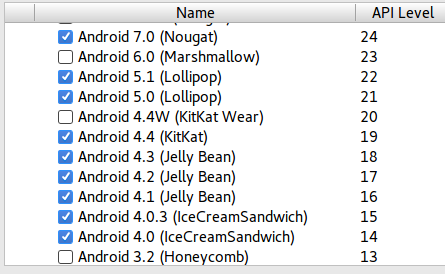
\includegraphics[scale=0.7]{assets/chpt_impl/sdks.PNG}
	\end{center}
\end{figure}

\subsection{Modifying and Compiling Rosandroid}
\label{impl:compiling_rosandroid}

Since the application developed in this thesis shall work on Android from versions beginning at 4.0.3 we have to modify the rosandroid code on one little detail to make everything work fine. In the created catkin workspace, go to the \textit{src} folder and clone the rosjava and rosandroid repositories there:
\begin{lstlisting}[caption={Cloning the rosandroid and rosjava repositories}]
git clone https://github.com/rosjava/rosjava_core.git
git clone https://github.com/rosjava/android_core.git
git clone https://github.com/rosjava/rosjava_messages.git
\end{lstlisting}

Then line 38 in the file
\begin{lstlisting}[numbers=none]
android_core/android_10/src/org/ros/android/RosActivity.java
\end{lstlisting}

has to be replaced by

\begin{lstlisting}[caption={Change to make to RosActivity.java},firstnumber=38]
public abstract class RosActivity extends android.support.v7.app.AppCompatActivity {
\end{lstlisting}

This gives us the ability to use the already-built features in rosandroid like the automatically displayed activity to connect to a ROS master and built-in node handling even in older Android versions. When changes are made, issue a \textit{catkin\_make} command in the catkin workspace's root directory. \textit{Rosjava} and \textit{rosandroid} will then be built from source and deployed to a \textit{Maven}\footnote{Maven is a dependency and package management system for Java libraries.} repository from where the binaries will be loaded by Android Studio on compile time.

\subsection{Starting the Environment}

To start up the development environment with the ROS master, the BioIK service and the \textit{rviz!} simulation of the robot, first the \textit{tams\_cml}\footnote{\url{https://gogs.crossmodal-learning.org/norman.hendrich/tams_cml}} and \textit{bio\_ik\_service}\footnote{\url{https://gogs.crossmodal-learning.org/philipp.ruppel/bio_ik_service}} packages has to be cloned into the catkin workspace, as well as the \textit{tams\_multitouch} package, which has to be copied into the workspace. After \textit{catkin\_make} was executed successfully, the programs are ready to be started. The following commands have to be entered in this order, but within different terminal sessions:
\begin{lstlisting}[caption={Commands to start up the development environment}]
roscore
roslaunch tams_multitouch demo.launch
roslaunch tams_f329 4_moveit.launch
rosrun bio_ik_service bio_ik_service
\end{lstlisting}

If interaction with the robot hardware is wanted, the corresponding programs and nodes have to be started according to the file \textit{tam\_cms/tams\_f329/README.txt} within the catkin workspace.

\section{User Interface}
\label{sec:impl:ui}

The user interface of the application was developed according to the considerations made in Chapter \ref{chap:concepts}. Additionally it turned out during development, that a basic tele-operation screen for the robot arm would be useful, that enables the user to bring the arm into a defined home position as well as doing simple step-wise manipulation to the robotic arm by moving the desired position of the hand palm by single small steps per button-press. The screen's layout and functionality is described in Section \ref{sec:impl:armteleop}.

The safety interlock button on all screens is immplemented using a \textit{FloatingActionButton}, a predefined control by Android which is designed to float in one corner of the screen above the rest of the screen's contents. To have the \textit{FloatingActionButton} work in the expected way, all screen contents have to be embedded into a \textit{CoordinatorLayout} container. The icon of the button has a \textit{Play} symbol in idle state, in activated state is shows a \textit{Pause} symbol until the button is released. The code to make the interlock button is described in Listing \ref{lst:impl:interlock}. It has to be inserted into the overridden \textit{onStart()} method in every Fragment of the application, in which the functionality shall exist - i.e. every page with controls for the robot.

\begin{lstlisting}[caption={Code for the interlock button}, label=lst:impl:interlock]
@Override
public void onStart() {
	super.onStart();
	
	final FloatingActionButton lockButton = ((FloatingActionButton)getView().findViewById(R.id.lockButton));

	lockButton.setOnTouchListener(new View.OnTouchListener() {
		boolean locked = true;
		
		@Override
		public boolean onTouch(View view, MotionEvent motionEvent) {
			switch(motionEvent.getAction())
			{
				case MotionEvent.ACTION_DOWN:
                        // Code to unlock robot operations
						lockButton.setBackgroundTintList(ColorStateList.valueOf(getResources().getColor(R.color.posOk)));
						lockButton.setImageResource(android.R.drawable.ic_media_pause);
				break;
				
				case MotionEvent.ACTION_UP:
					// Code to lock robot operations
					lockButton.setBackgroundTintList(ColorStateList.valueOf(getResources().getColor(R.color.posNOk)));
					lockButton.setImageResource(android.R.drawable.ic_media_play);
				break;
			}			
			return true;
		}
	});
	
	// ... more code for onStart()
}
\end{lstlisting}

\subsection{Synergy Pages}

\begin{figure}
	\caption{The synergy control screen\label{fig:ui:syn}}
	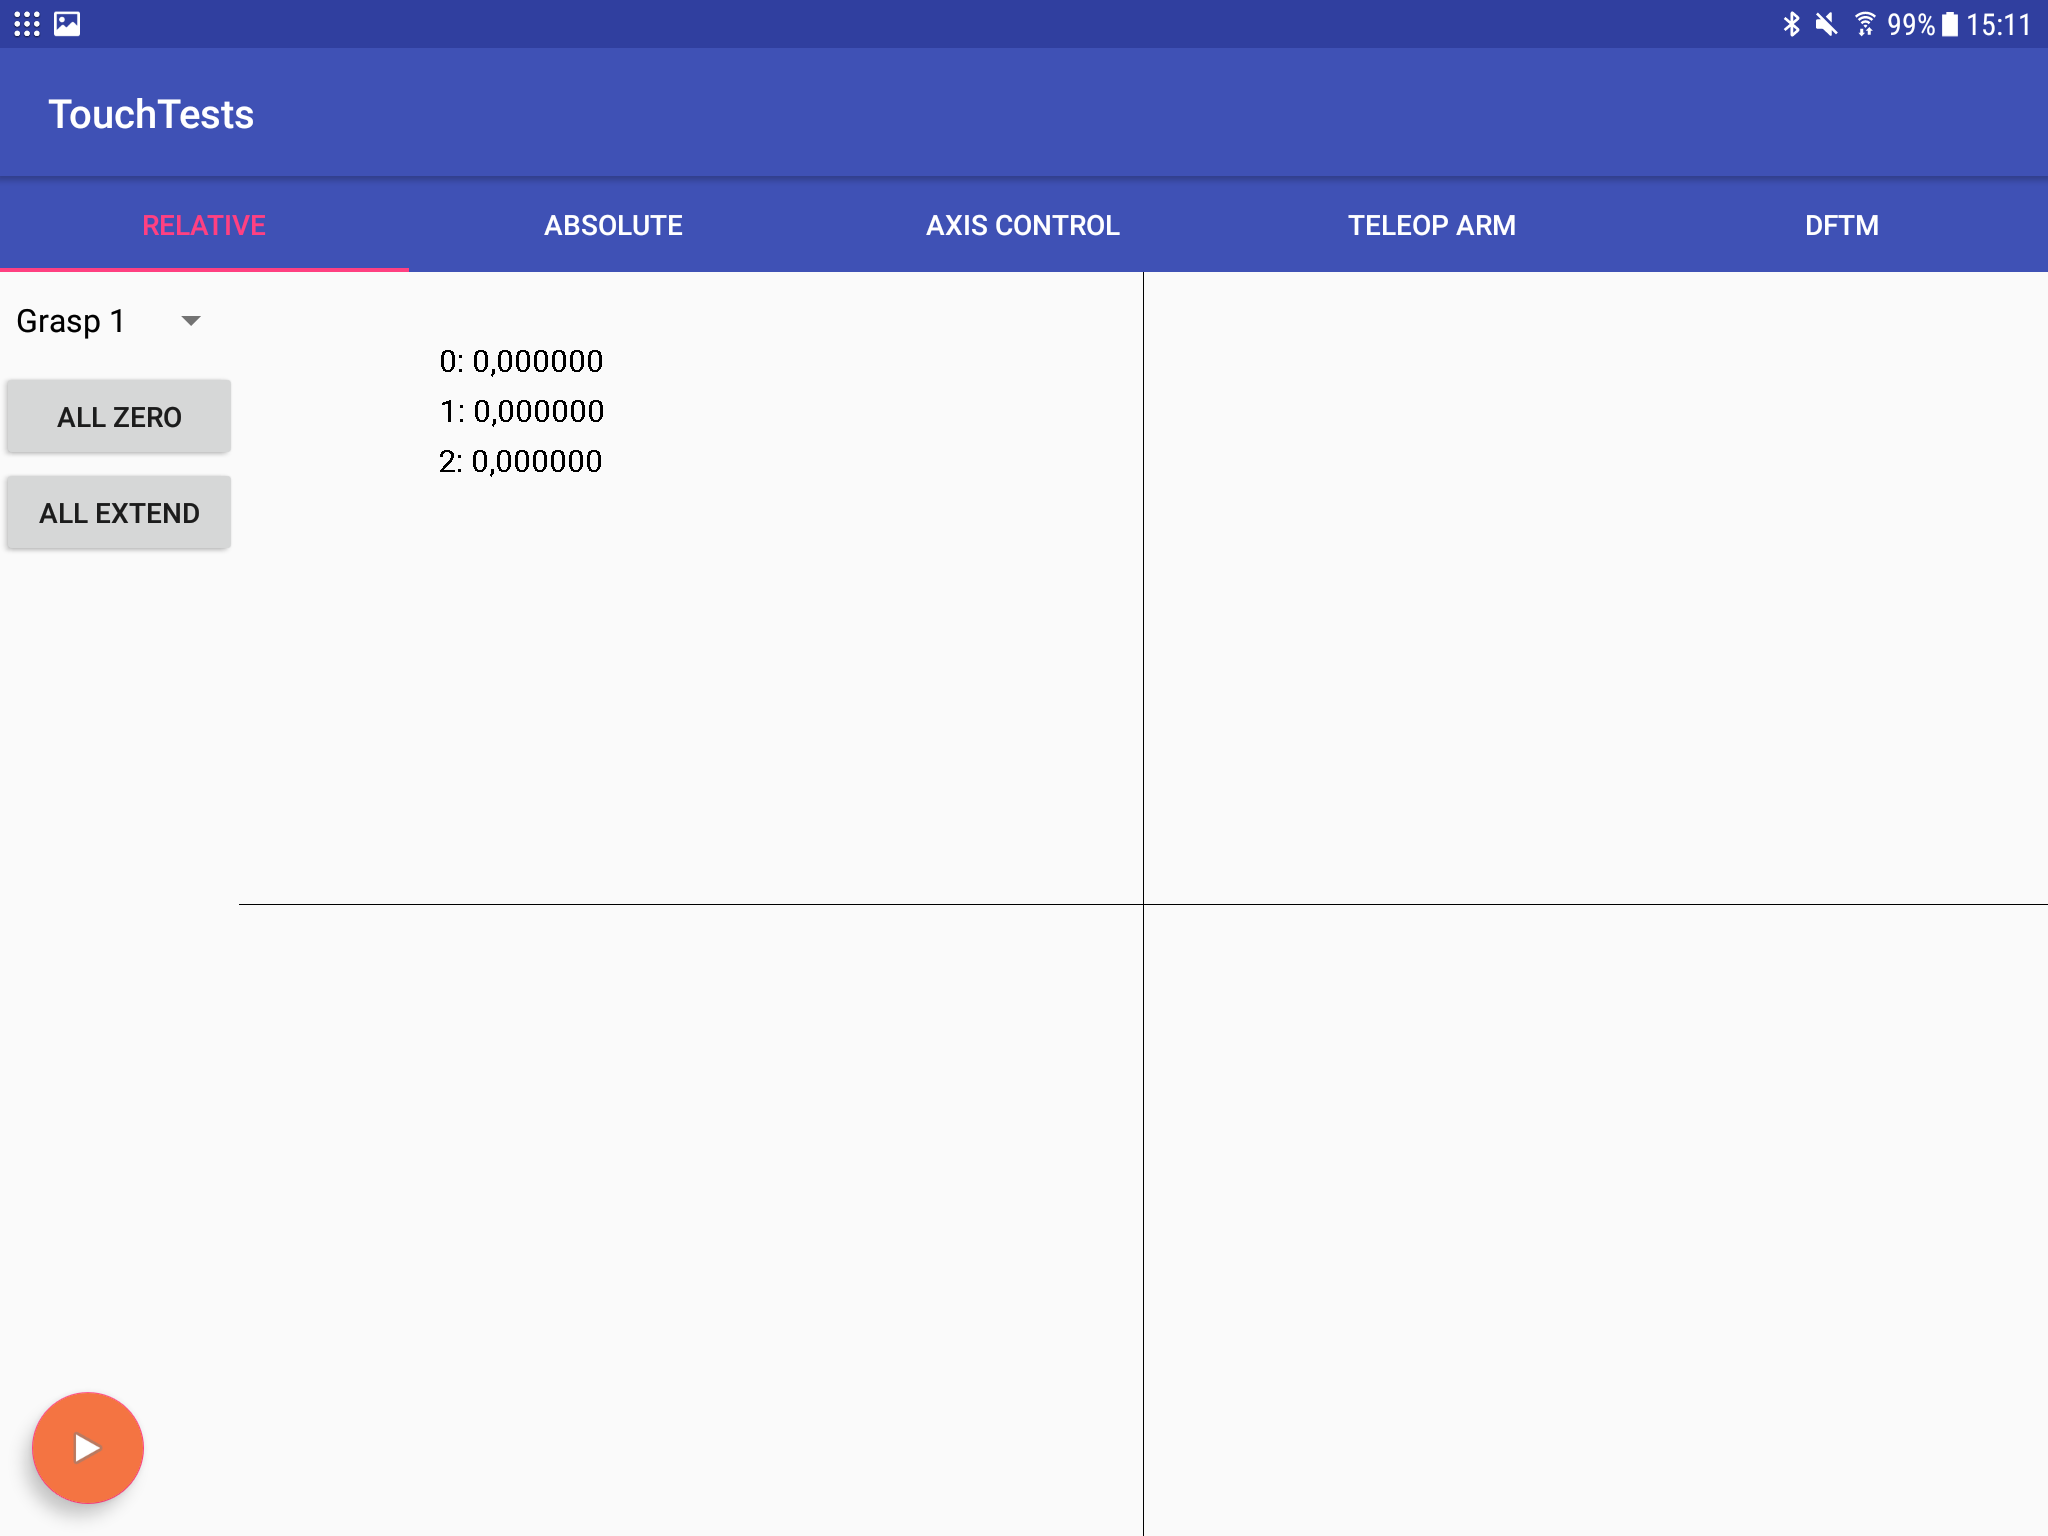
\includegraphics[width=\linewidth]{assets/chpt_impl/syn_blank}
\end{figure}

\begin{figure}
	\caption{display of a two-pointer and a three-pointer gesture on the synergy screen\label{fig:ui:syngest}}
	
	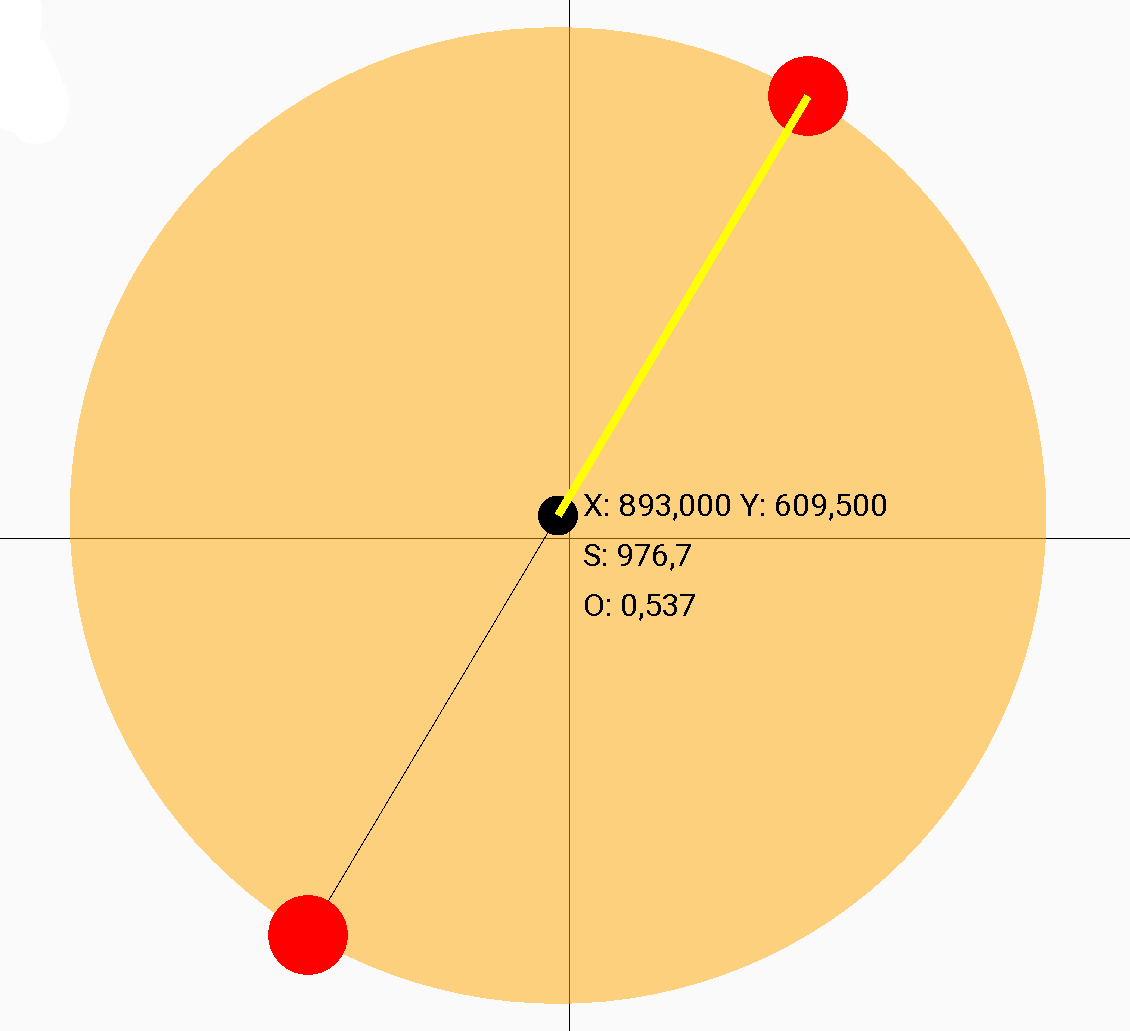
\includegraphics[width=0.5\linewidth]{assets/chpt_impl/syn_2touch}
	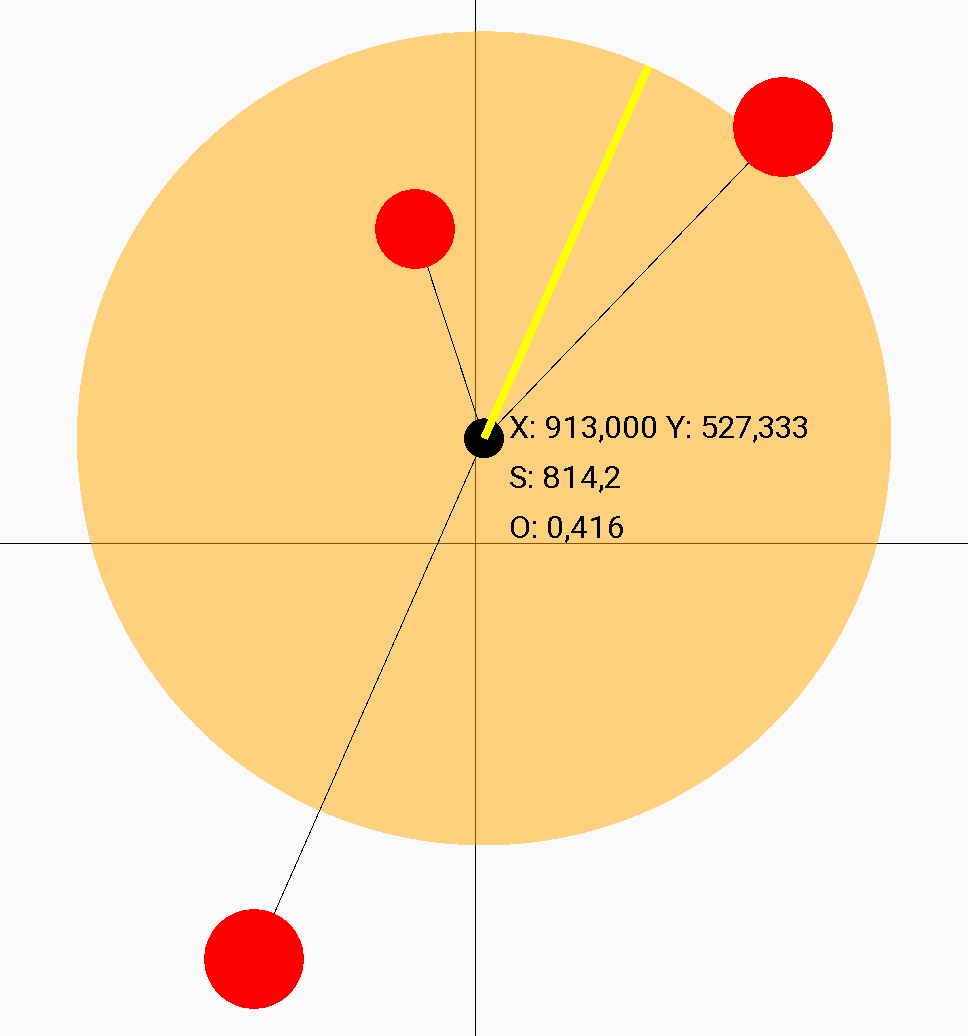
\includegraphics[width=0.5\linewidth]{assets/chpt_impl/syn_3touch}
\end{figure}

The synergy pages are implemented as a mostly blank white page, with a small drop-down control on the left to select the synergy that shall be controlled, as well as a two buttons to set all amplitudes to a known state (i.e. either all zero or all 50). The values of all three controllable amplitudes are displayed in the upper left corner of the control area. The screens for absolute and relative control look the same, which mode is active can be seen in the upper bar with the tab controls. Two lines determine the middle of the control area, which is important for the absolute approach, as the absolute placement of a gesture is important. Figure \ref{fig:ui:syn} gives an impression of how the screen looks on the tablet computer.

Figure \ref{fig:ui:syngest} shows how a two-pointer and a three-pointer gesture is displayed on the synergy pages. While each pointer is marked by a red circle, the center (i.e. the position) of a gesture is displayed as a small black circle, with all pointers being connected to the center by a black line. The orange circle gives an impression of the calculated size of a gesture while the yellow line within the orange circle points in the direction of the orientation which was calculated for a gesture. The calculated values are also displayed in clear text next to the center of a gesture. This is done mainly for debugging purpose, but may also give an interesting insight into the state of a gesture, for example for training purposes. Note that the orientation is not given in degrees, but in radians.

\subsection{Direct Fingertip Mapping (DFTM) Page}

Figure \ref{fig:ui:dfmt} gives an overview of how the DFTM page looks like. It has even less contents than the synergy pages, as no selection has to be made for the current implementation of the DFTM approach. In later iterations it would be sensible to add controls to move the base of the currently workspace on which the fingertips are mapped. As this is not implemented within this thesis, no such controls are displayed. In the same figure an example of how touch pointers are displayed is given for three points. Next to each pointer the name of the link controlled by this pointer is displayed, as well as the coordinates in screen coordinates (i.e. pixels) and world coordinates (i.e. centimeters), both originating in the top-left corner of the white control area. As described more detailed in Section \ref{sec:impl:dfmt}, the pointers are assigned to the links they control in the order in which they are placed on the screen.
If a finger is lifted from the screen (i.e. the touch pointer is de-registered by the Android operating system), one of the following two actions will be performed:
\begin{itemize}
	\item If a pointer of a finger laid down on the screen later than the pointer removed is still present, the pointer is marked as \textit{not present}. Its position does not change, but is still included in IK requests. 
	\item If no such pointer exists, i.e. the lifted pointer was the last present pointer if order of occurrence, it is removed and all pointers laid down after the current one but marked as \textit{not present} are also removed and not included in IK requests anymore.
\end{itemize}

A pointer which is marked as \textit{not present} is displayed as an unfilled circle with a black border (refer to Figure \ref{fig:ui:dfmt_lift} for an example). Once the user places a finger within the black circle, it is registered as this pointer again and the pointer is marked as \textit{present}.

\begin{figure}
	\caption{\label{fig:ui:dfmt}The DFTM screen with three pointers}
	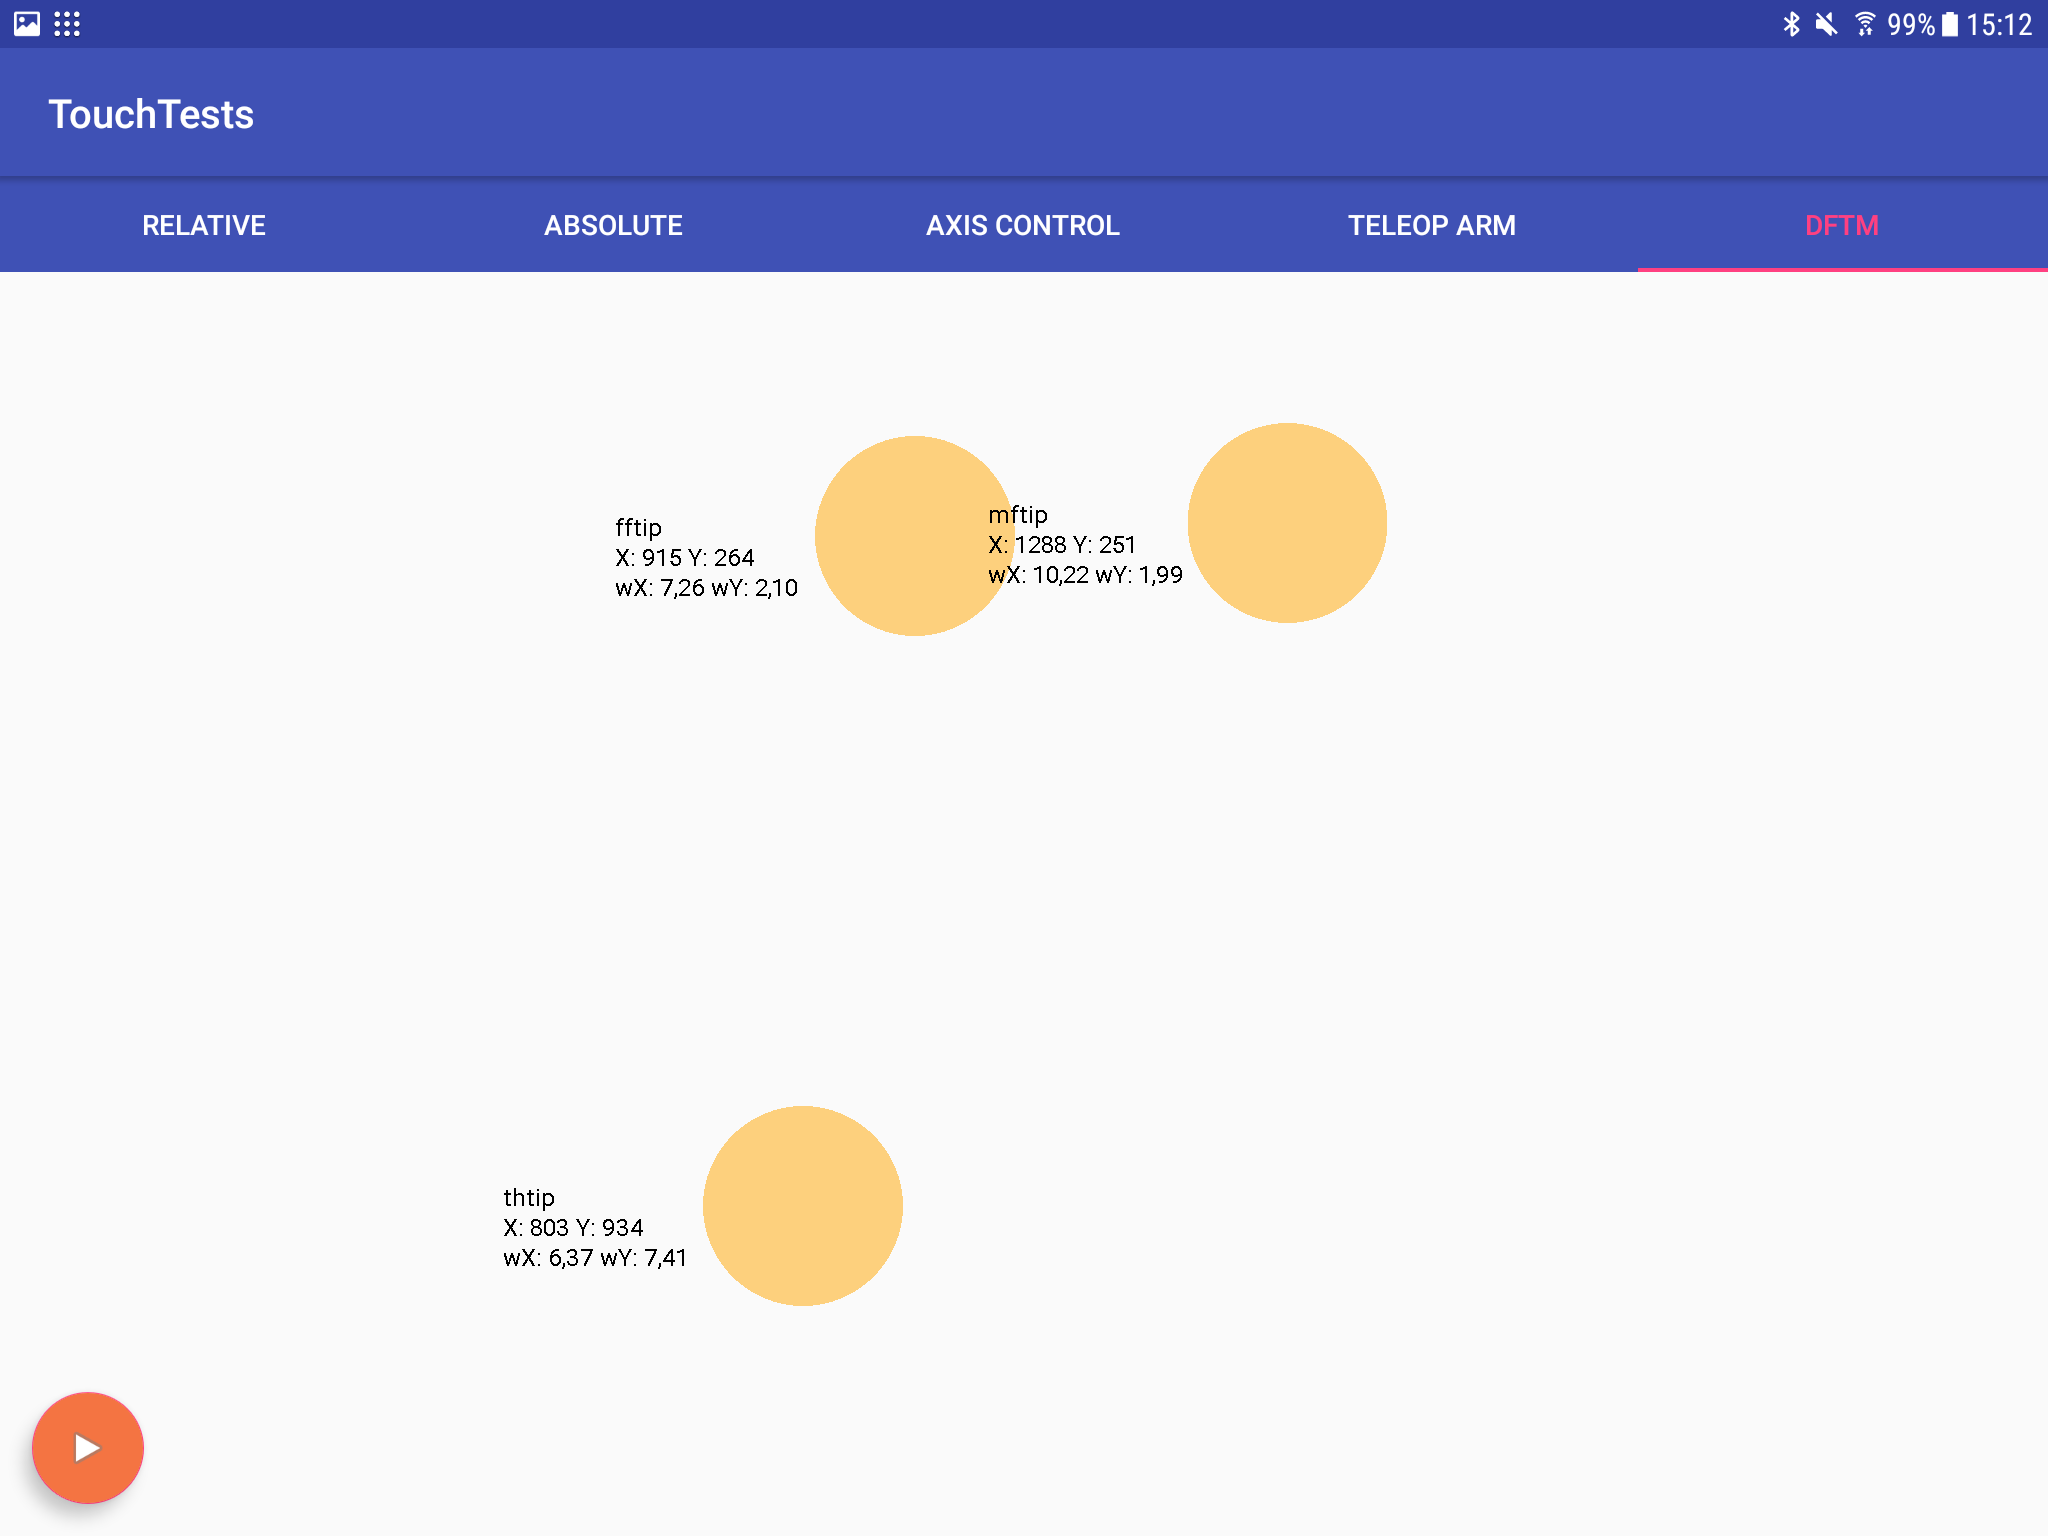
\includegraphics[width=0.9\linewidth]{assets/chpt_impl/dftm}
\end{figure}

\begin{figure}
	\caption{\label{fig:ui:dfmt_lift}The DFTM screen with three pointers, of which one is currently not laid on the screen}
	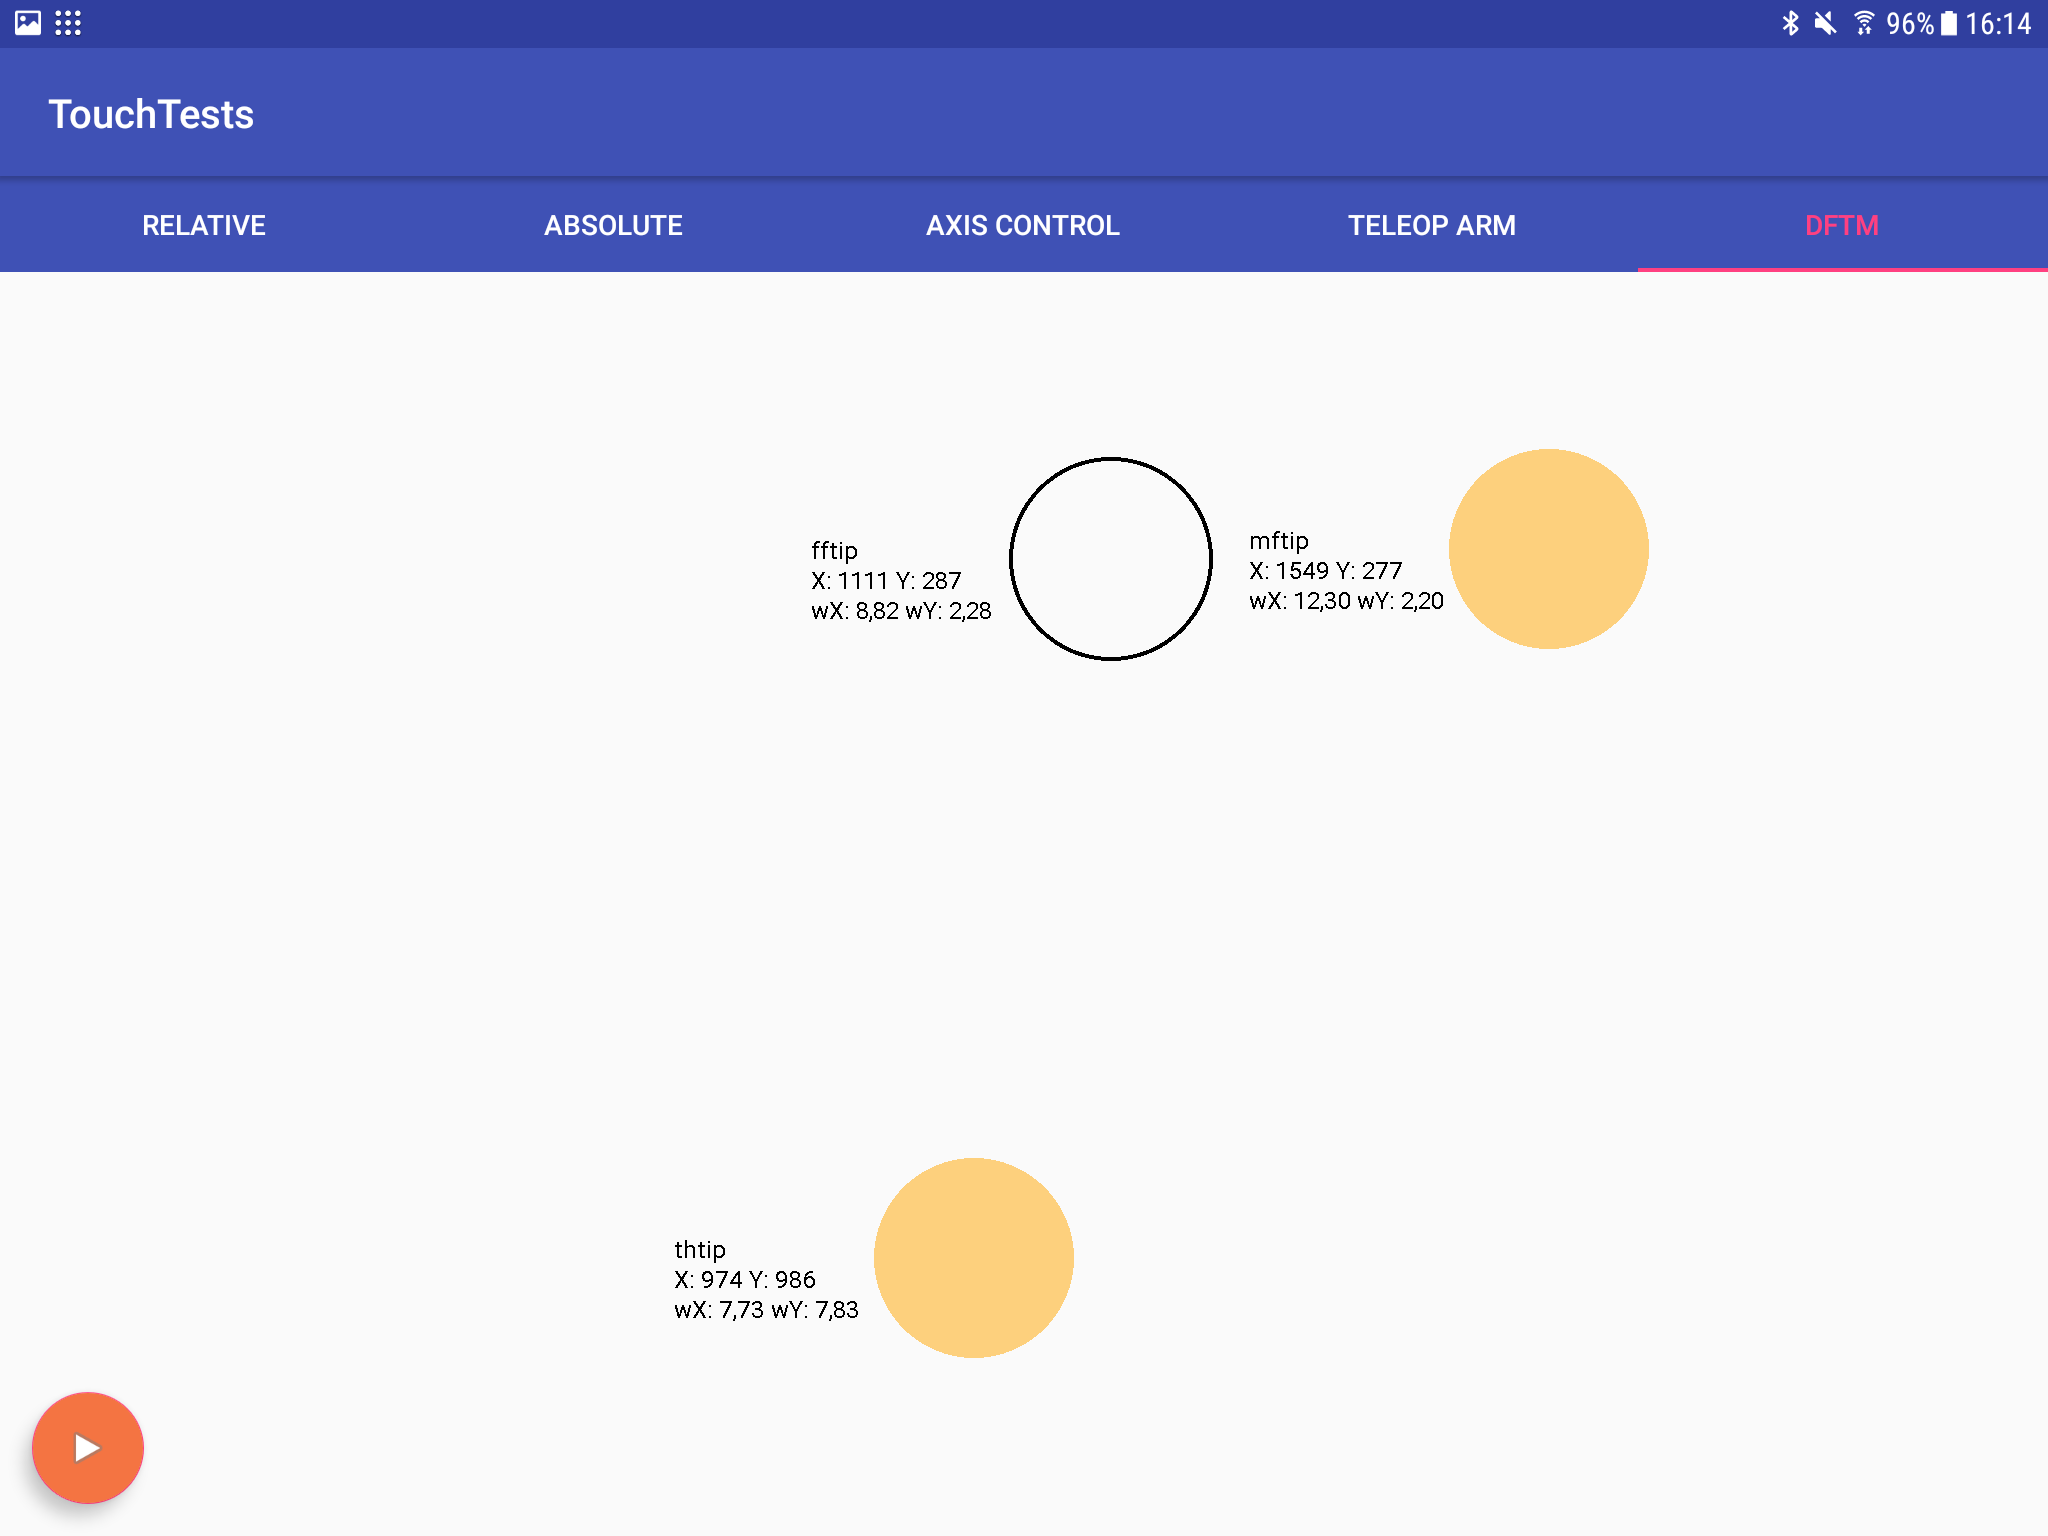
\includegraphics[width=0.9\linewidth]{assets/chpt_impl/dftm_lifted}
\end{figure}

\subsection{Axis Control Page}

The axis control page consists of many \textit{single axis controls} (one for each axis or joint available in the robot, see Figure \ref{fig:ui:axiscontrol}), which -- as defined earlier -- possess two buttons, one to increase and one to decrease the position of the axis or joint. Between those two buttons the target value is displayed (on the top in bold), as well as the currently measured value as received from the robot (in the bottom). The colour between the buttons indicates the magnitude of difference between the target value and the currently measured value as described in Section \ref{sec:conc:axiscontrol}. Axis control widgets for axes that are not controllable (i.e. the first one for every finger except the thumb) have their buttons greyed out and are thus only there to display the current value of the axis.

Two extra buttons are placed on the screen, one labelled \textit{Stop} and one \textit{All Zero}. These buttons are mapped to functionality explained in Section \ref{sec:impl:axism:stop}. The former sets all target values to zero, while the latter copies all currently measured values into the target value, causing the robot to stop all movements.

\begin{figure}
	\caption{\label{fig:ui:axiscontrol}The axis control page}
	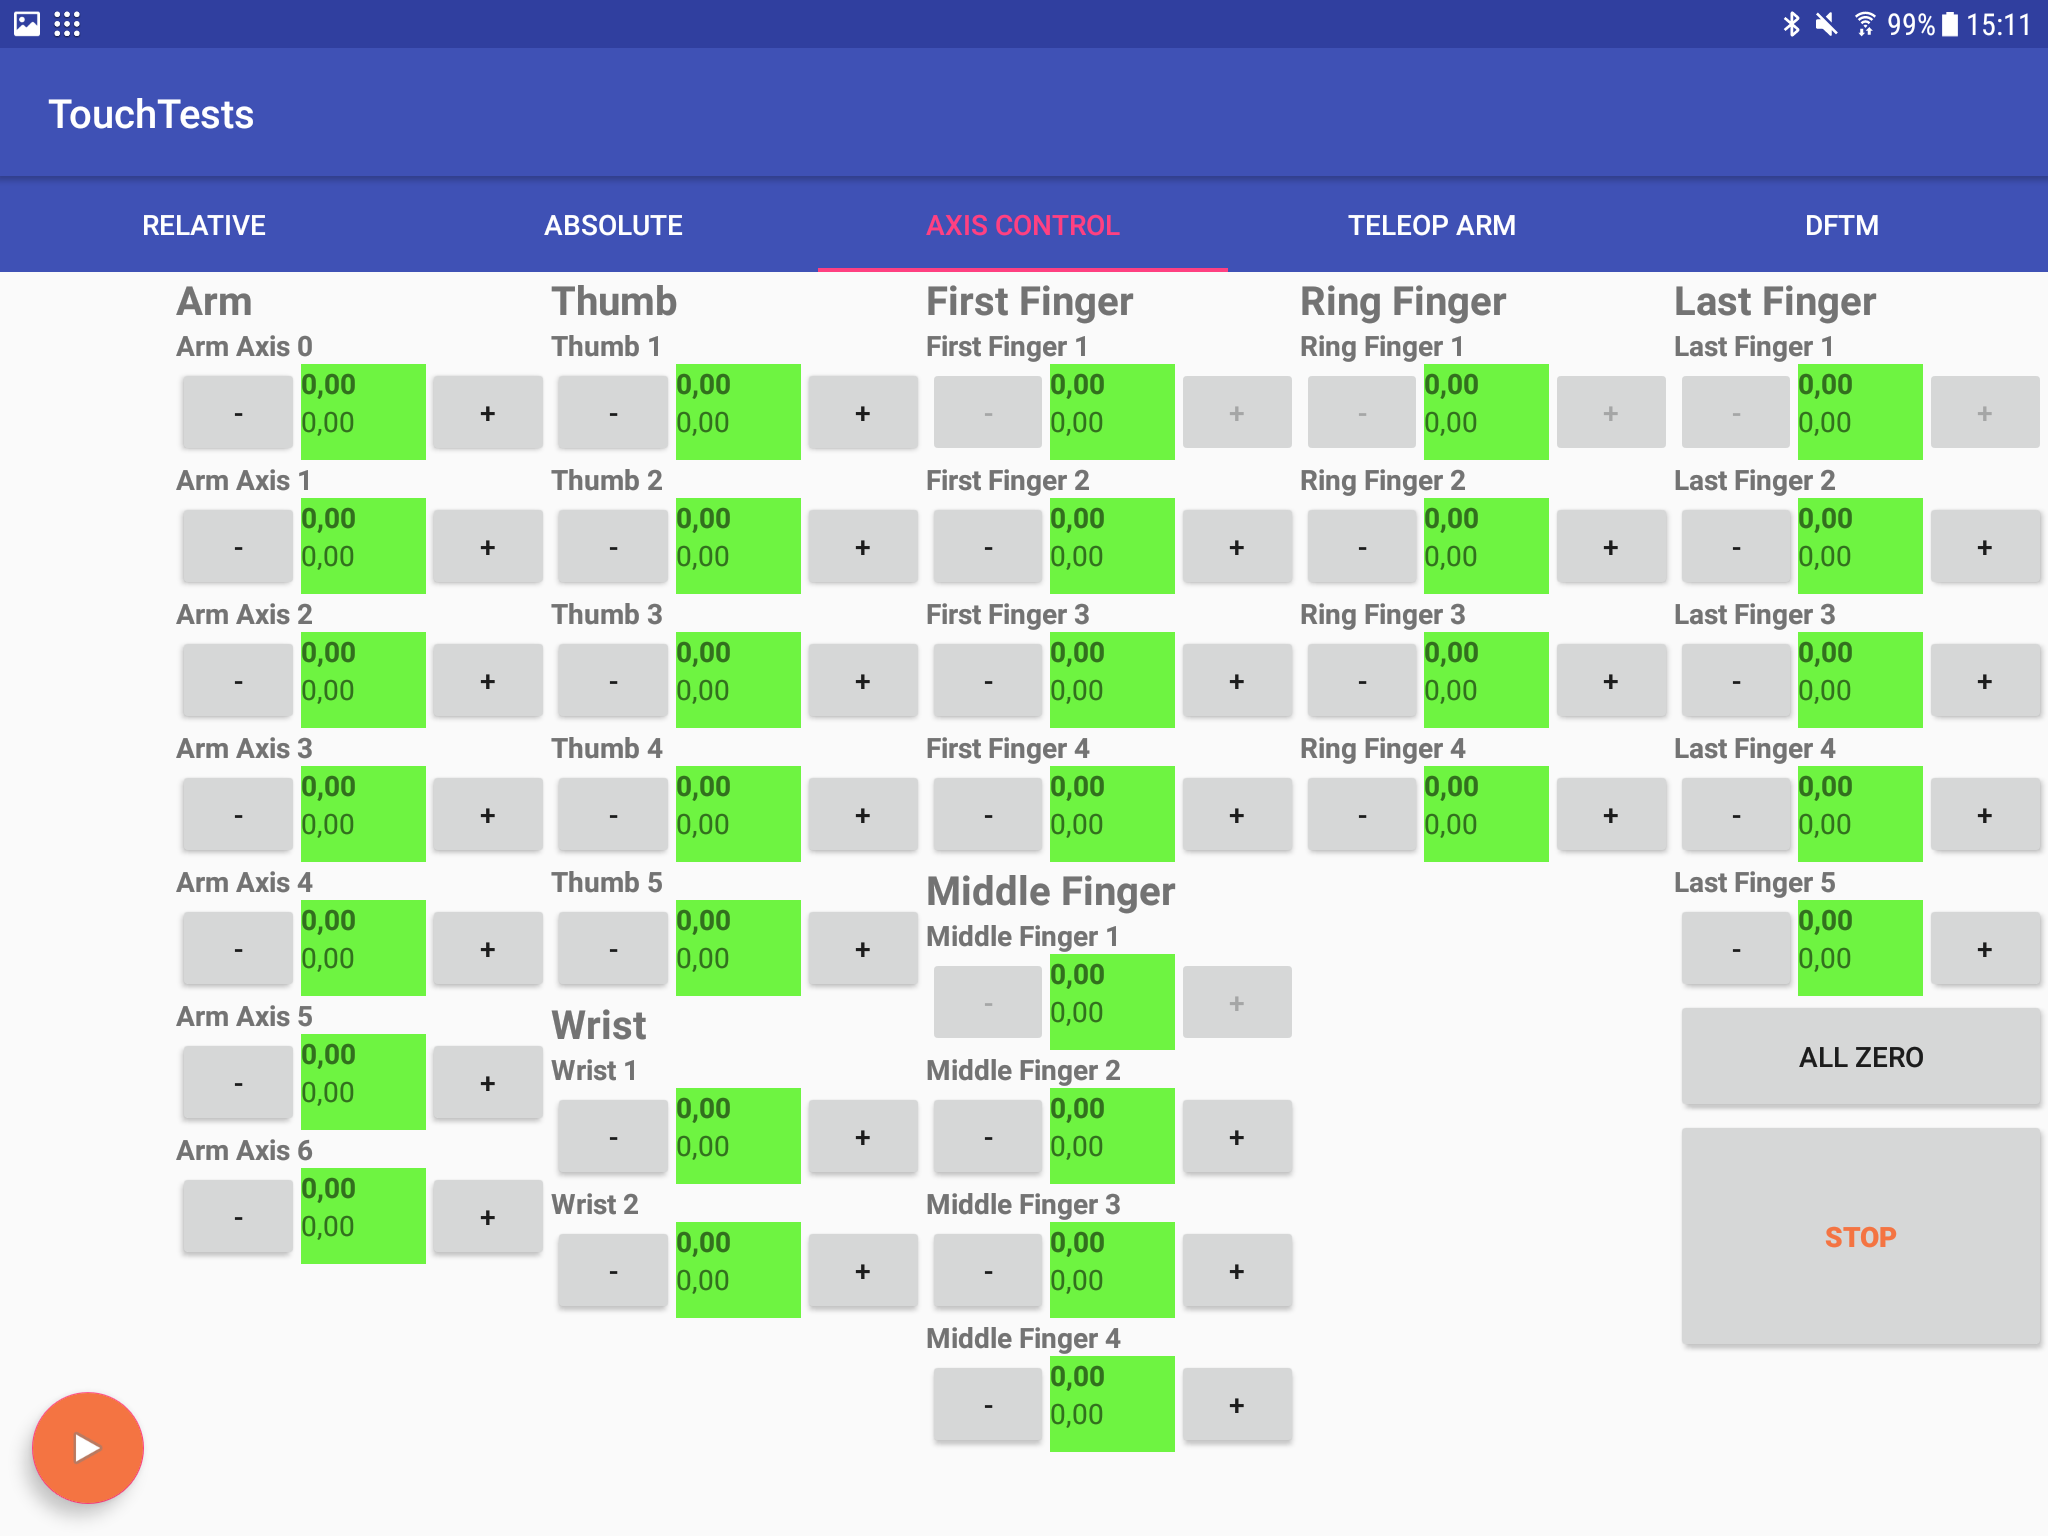
\includegraphics[width=0.9\linewidth]{assets/chpt_impl/axis_control}
\end{figure}

\subsection{Arm Tele-Operation Page}
\label{sec:impl:armteleop}

\begin{figure}
	\caption{\label{fig:ui:teleop}The arm tele-op page}
	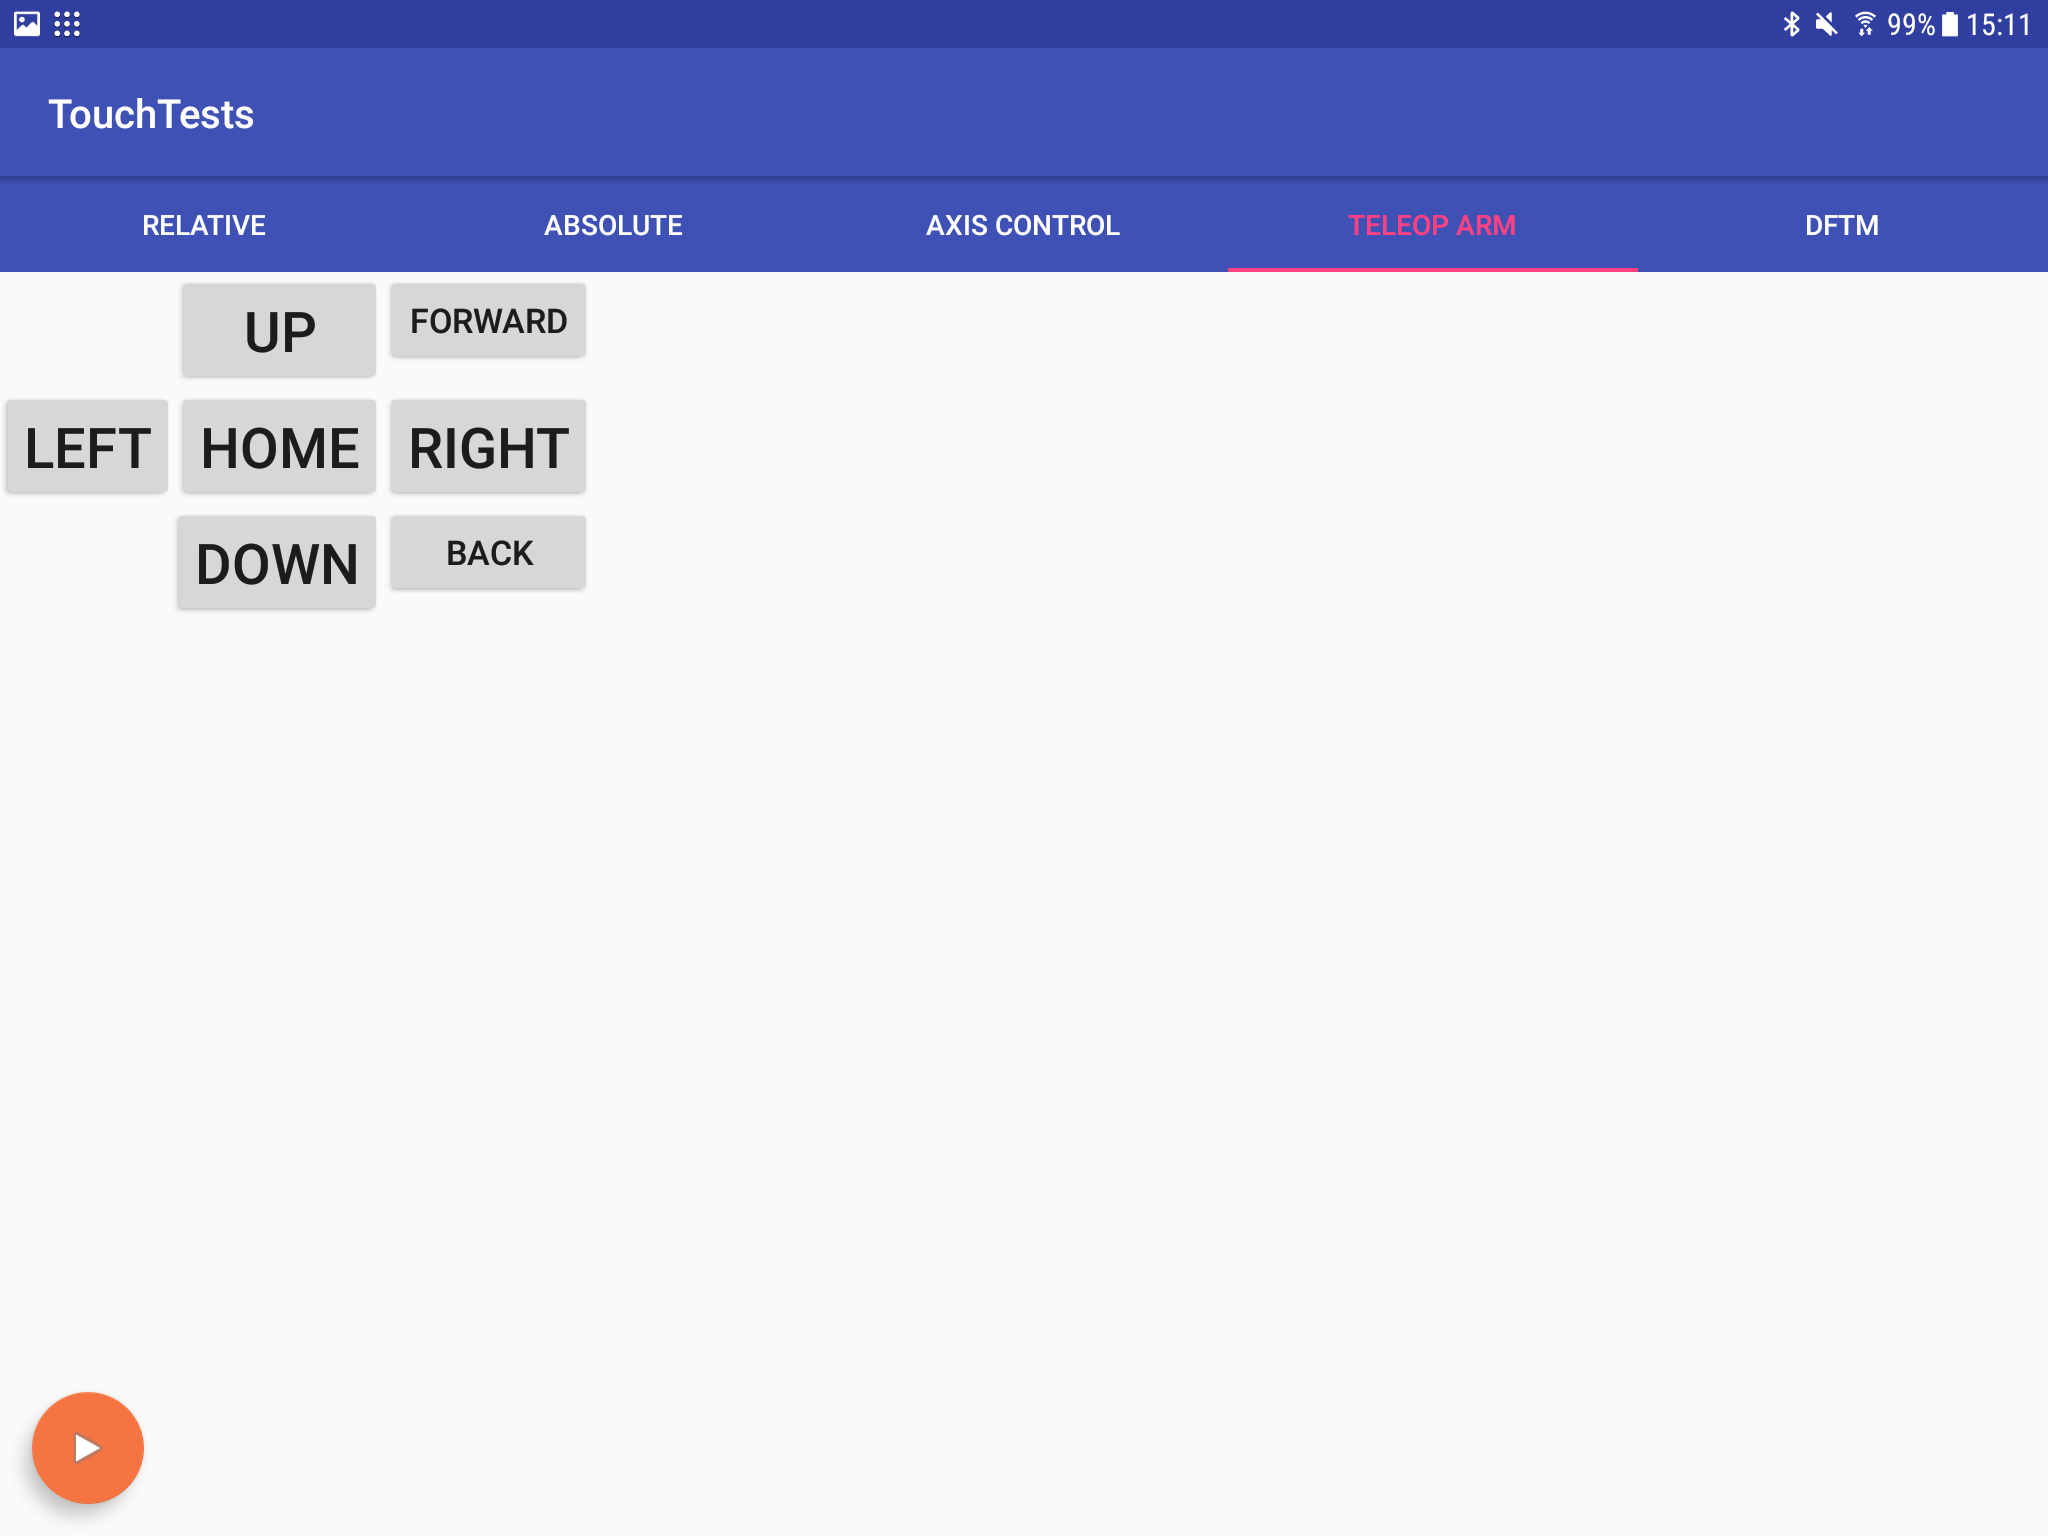
\includegraphics[width=0.9\linewidth]{assets/chpt_impl/teleop}
\end{figure}

As a last page, the arm tele-op page servers as a remote control to move the arm in Cartesian space. The functionality of the \textit{CartesianArmManager} described in Section \ref{sec:impl:armcontrol}. It is important to note that the wording \textit{left, right, forward, backward} are relative to the operators point of view, as standing in front of the robot. Each button press moves the palm of the robot by one centimeter into the desired direction. A press on the \textit{Home} button brings the robot into a home position, which is located directly in front of the robot at the border of the table approximately 20cm above the plate. This page was implemented for testing reasons, but comes in handy when using the synergy approaches, as the arm should be moved into the \textit{Home} position first before using the gesture control. Doing this using this page is easier than moving every joint on its own using the axis control page. Figure \ref{fig:ui:teleop} gives an impression of the page.

\section{ROS integration}

Thanks to \textit{rosandroid} it is easy to integrate ROS into an Android application. When the libraries are included in the project the main thing to change is that the main activity has to inherit from \textit{RosActivity} instead of the plain Android \textit{Activity} class.

\begin{lstlisting}[caption={Changes to MainActivity}, escapechar=&]
public class MainActivity &\textbf{extends RosActivity}& {
	//...
}
\end{lstlisting}

\begin{wrapfigure}[14]{R}{0.60\linewidth}
\caption{\label{fig:impl:masterchooser}The rosandroid master chooser activity}
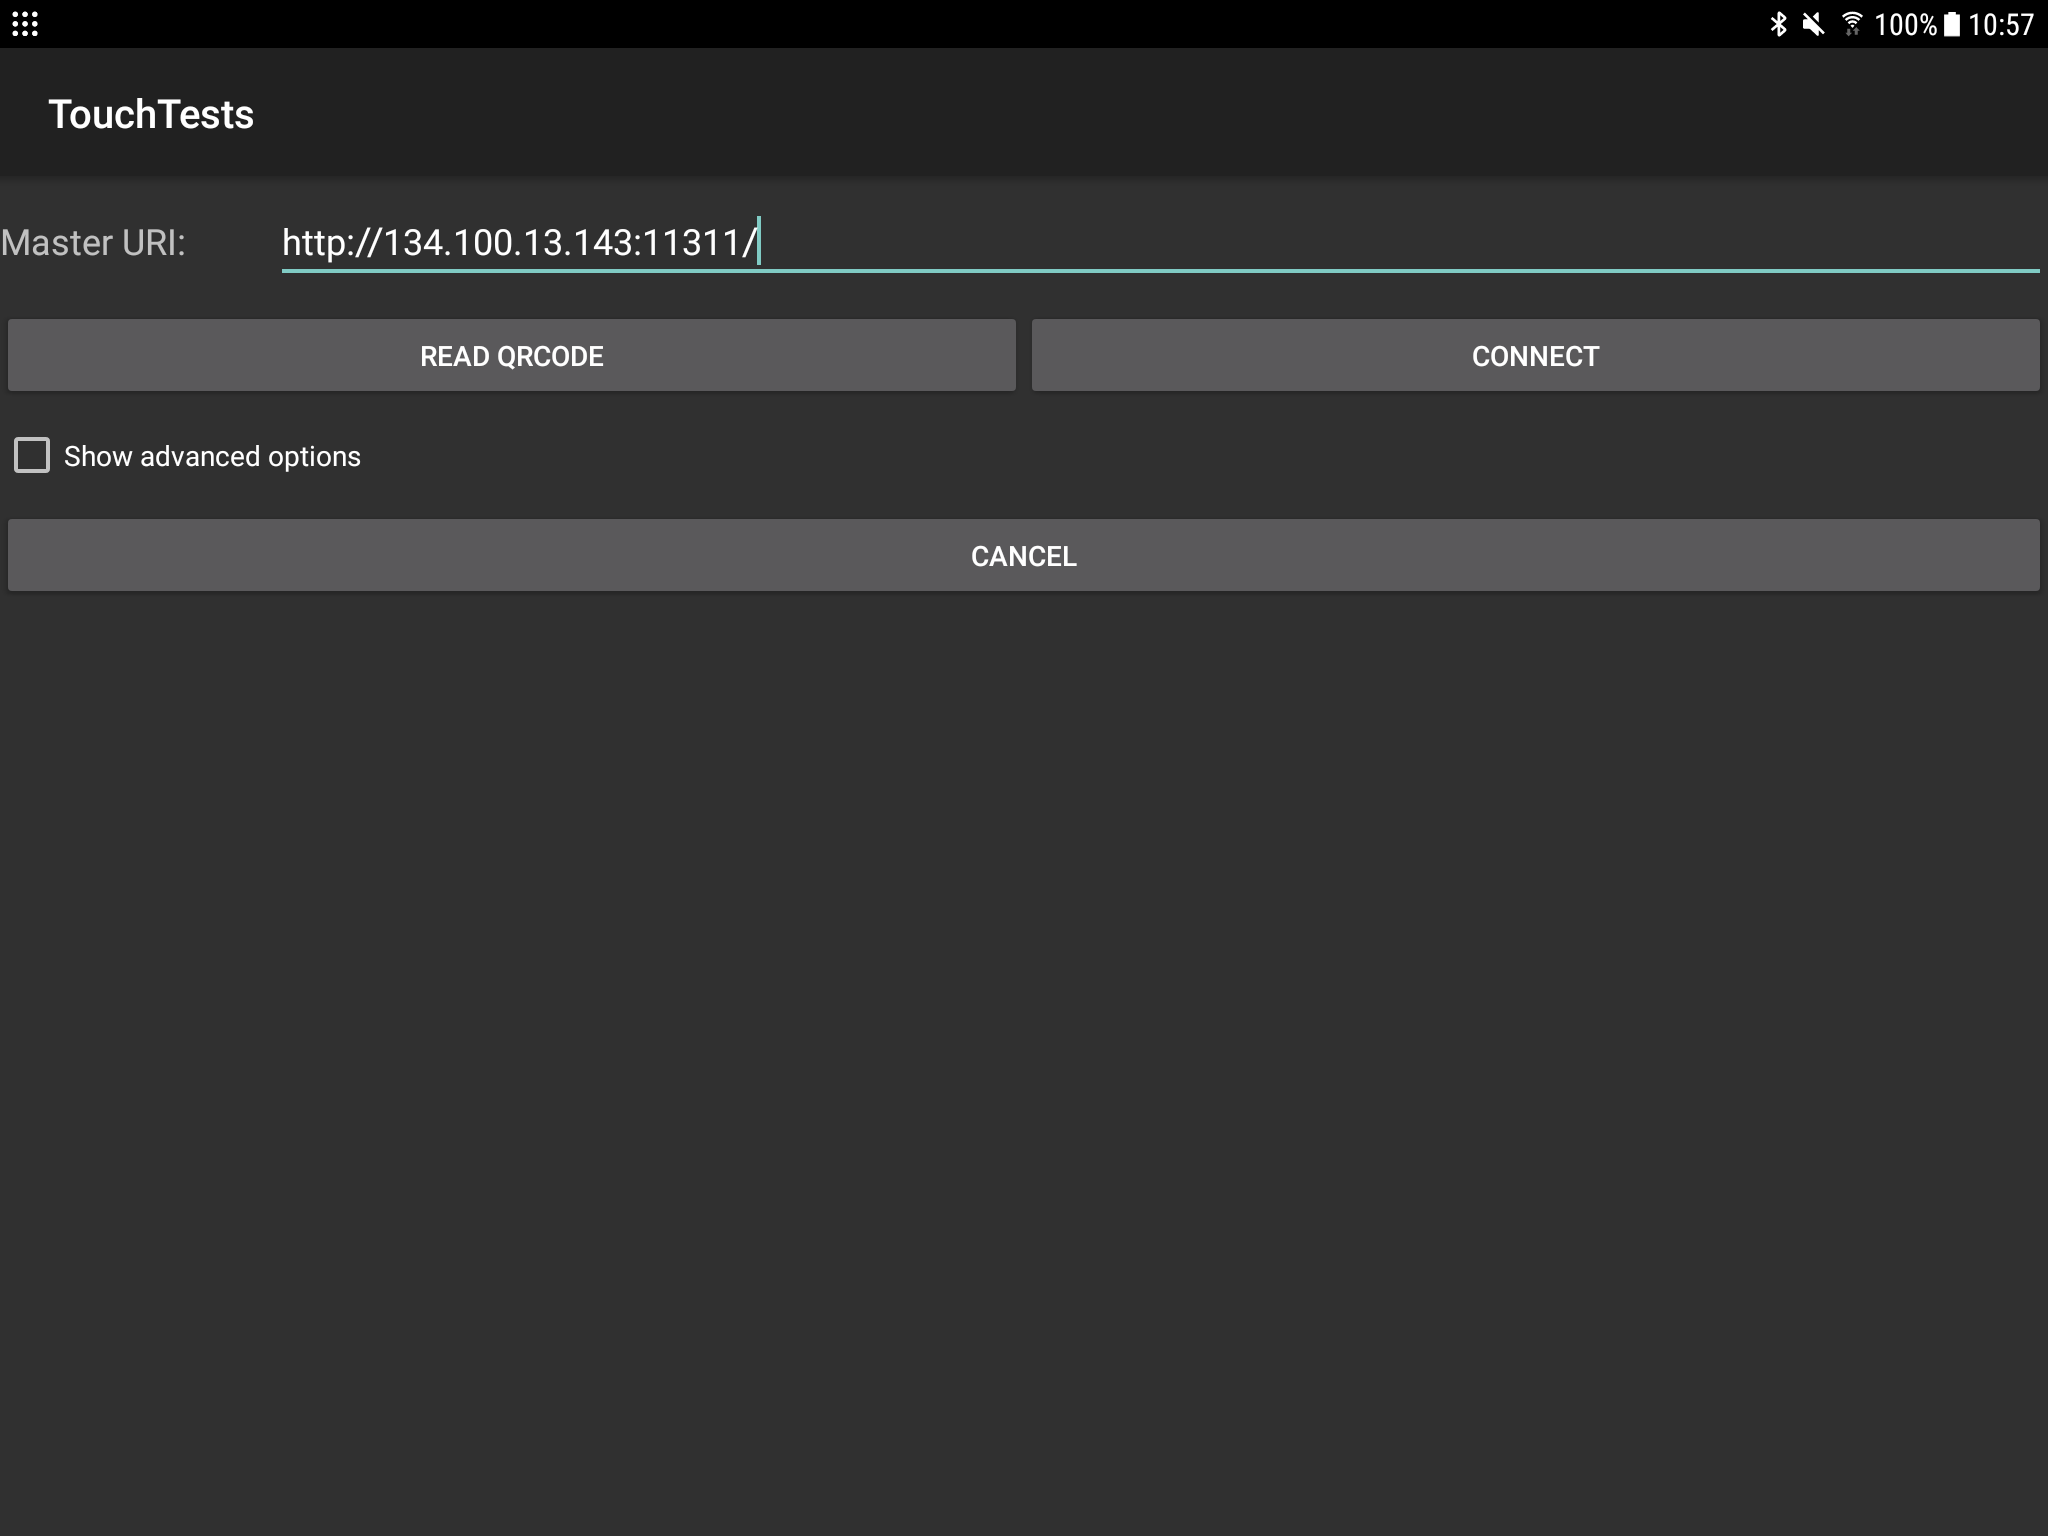
\includegraphics[width=\linewidth]{assets/chpt_impl/masterchooser}	
\end{wrapfigure}

After this change was made, the \textit{RosActivity} implementation takes care about multiple things, beginning with showing a \textit{master chooser}  activity, in which the user can connect to a ROS master node, to handling all connection lifetime events of ROS parts. The \textit{master chooser} activity (see Figure \ref{fig:impl:masterchooser}) lets the user connect to an existing ROS master node. Additionally, it gives the Android application the opportunity to create a dedicated master node on the device itself. As this could affect the overall performance of the application and a lot of functionality has to be run on a more powerful machine, the ROS master is started on a dedicated computer and the Android application connects to this existing master node.

\textit{RosActivity} is an abstract class. To implement it, the \textit{init()} method has to be overriden by inheriting classes. This method is called once the connection to the ROS master node was established and custom nodes can be initialized and connected. All other initialization steps regarding the implemented ROS nodes should also be done here. As shown in Listing \ref{lst:impl:rosconn}\footnote{Information on how to initialize ROS applications was taken from an official rosandroid example found at \url{https://github.com/rosjava/android_core/blob/kinetic/android_tutorial_pubsub/src/org/ros/android/android_tutorial_pubsub/MainActivity.java}}, first an instance of the \textit{C5LwrNode} is created and then assigned to all instances that consume functionality of it (\textit{AxisManager}, \textit{CartesianArmManager}, \textit{DfmtProxy}). After all this is done, the node is registered with the ROS master node. Details on the initialization of the \textit{C5LwrNode} node can be found below in this section. In theory, multiple nodes can be started and registered with the master within one application.

\begin{lstlisting}[caption={Initialization of the ROS connection}, label={lst:impl:rosconn}]
@Override
protected void init(NodeMainExecutor nodeMainExecutor) {
	axisManager = AxisManager.getInstance();
	
	node = new C5LwrNode("/joint_states", "/hand/joint_goals", "/lwr/jointPositionGoal");
	node.addJointDataListener(axisManager);
	
	axisManager.setRobotNode(node);
	CartesianArmManager.getInstance().setNode(node);
	DftmProxy.getInstance().setNode(node);

	NodeConfiguration cfg = NodeConfiguration.newPublic(getRosHostname(), getMasterUri());
	nodeMainExecutor.execute(node, cfg);
}
\end{lstlisting}

\subsection{The C5LwrNode Class}

The class \textit{C5LwrNode} inherits from \textit{AbstractNodeMain}, which already offers the very basic lifetime functionality of a ROS node. Some methods have to be implemented by the developer, like \textit{getDefaultNodeName()}, which determines the name of the ROS node as it is registered with the ROS master. In the \textit{onStart()} method, all start-up procedures are implemented, like registering topic subscriptions as well as creating publishers and \textit{service clients}. Within the \textit{onShutdown()} method, all resources created before (subscribers, publishers, service clients) shall be closed and deleted to ensure a clean de-registration from the ROS master and a clean shut-down of the application. The start-up code for the ROS node can be seen in Listing \ref{lst:impl:c5lwrnode}.

\begin{lstlisting}[caption={Startup of the C5LwrNode}, label=lst:impl:c5lwrnode]
@Override
public GraphName getDefaultNodeName() {
	return GraphName.of("ba_android/c5lwrnode");
}

@Override
public void onStart(ConnectedNode connectedNode) {
	cNode = connectedNode;
	handJointStatePub = connectedNode.newPublisher(handPublishTopic, JointState._TYPE);
	armJointStatePub = connectedNode.newPublisher(armPublishTopic, RMLPositionInputParameters._TYPE);

	jointStateSubsc = connectedNode.newSubscriber(subscribeTopic, JointState._TYPE);
	jointStateSubsc.addMessageListener(/* ... */);

	try {
		ikService = connectedNode.newServiceClient("/bio_ik/get_bio_ik", bio_ik_msgs.GetIK._TYPE);
	} catch (ServiceNotFoundException e) {
		ikService = null;
		e.printStackTrace();
	}
}
\end{lstlisting}

The methods that are used to offer the functionality of the \textit{C5LwrNode} are denoted in Listing \ref{lst:impl:c5lwrik}. Because arm and hand joints have to be published to different topics, the \textit{handleJointData()} method calls either \textit{publishHand()} oder \textit{publishArm()}, depending on the parameter \textit{jointType} which is passed by the caller indicating the type of the joint data given. The two methods to request IK solutions from the BioIK service are relatively similar, as both initialize the request with the current robot state passed as a parameter and add a \textit{MinimumDisplacementGoal} to hint the IK solver that a solution is desirable where the least possible movement in all axes is done. The number of attempts is set to $1$, the time-out to find a solution is set to $10ms$ for the palm position and $500ms$ for the fingertip positions. The main difference is that, while for the palm only one \textit{PoseGoal} is added, containing the desired pose of the palm constructed by the x, y, z position and \textit{Quaternion} rotation as passed by the caller, in the method to get a solution for multiple fingertips one \textit{PositionGoal} is added for each fingertip as well as an \textit{OrientationGoal} to have the palm of the robotic hand always point in the same direction. In \textit{GetIKJointsFingertips()}, the \textit{fingertips} parameter contains a map with the link names (e.g. \textit{fftip}, \textit{thtip}...) as key values and the desired 3-dimensional position of the link.

\begin{lstlisting}[caption={C5LwrNode interface},label=lst:impl:c5lwrik]
public class C5LwrNode extends org.ros.node.AbstractNodeMain implements RobotJointDataReceiver {
	private void publishHand(HashMap<String, Double> data);
	private void publishArm(HashMap<String, Double> data);
	
	@Override
	public void handleJointData(int jointType, HashMap<String, Double> data);
	
	public void GetIkJointsPalm(Map<String, Double> currentState, 
		String[] lockedAxes, 
		double x, double y, double z, 
		double rotx, double roty, double rotz, double rotw,
		ServiceResponseListener<GetIKResponse> hdl);
	
	public void GetIKJointsFingertips(Map<String, Double> currentState,
		Map<String, PointInSpace> fingertips, 
		ServiceResponseListener<GetIKResponse> hdl);
}

\end{lstlisting}

\section{The AxisManager}

The most important and most central functionality of the overall application is offered by the \textit{AxisManager} class. It is responsible for holding the current joint angles for all joints in memory, as well as the current target values along multiple other bits of information about each axis or joint. Joints are more generically called \textit{axis} within the \textit{AxisManager}, so this wording will be adopted in the rest of this section.

\subsection{AxisInformation}

All information about an axis is stored in a \textit{AxisInformationImpl} object. This class implements the \textit{AxisInformation} interface, which is returned when axis information shall be given to callers in a read-only manner. The \textit{AxisInformation} interface is given in Listing \ref{lst:impl:axisinformation}. All the information stored about an axis is accessible here. In particular, this is: 
\begin{itemize}
	\item The identifier of an axis, i.e. a string literal containing the name at which The axis or joint is known to the ROS nodes.
	\item The maximum speed the axis may move at.
	\item The target value to which the axis shall be currently moved.
	\item The value representing the axis' current position.
	\item The value representing the axis' \textit{current target value} (see Section \ref{sec:impl:axismovements} for details).
	\item The minimum and maximum values the axis may have as position value.
	\item flags indicating whether the axis is enabled and moving.
	\item An integer representing the type of an axis. Allowed types are \textit{JointType.ARM} and \textit{JointType.HAND}.
\end{itemize}

\begin{lstlisting}[caption={The AxisInformation interface}, label=lst:impl:axisinformation]
public interface AxisInformation {
	String getIdentifier();
	
	double getMaxSpeed();
	double getTargetValue();
	
	double getMaxValue();
	double getMinValue();
	double getCurrentTargetValue();
	double getCurrentValue();
	boolean isMoving();
	double getSpeed();
	boolean isEnabled();
	int getJointType();
}
\end{lstlisting}

All the information is held within the \textit{AxisManager}, referenced by the axis identifier. Manipulation of the data is only done through calls to the \textit{AxisManager}, to give it full control about what happens with all axes. The difference between \textit{AxisInformation} and the concrete implementation \textit{AxisInformationImpl} is, that the implementation has a setter function for every property. All calculations are done within the \textit{AxisManager} itself.

\subsection{AxisManager Timer Tick}

The \textit{AxisManager} is designed to work fully asynchronous. All information about axes' target values is stored in the according \textit{AxisInformation} object, but only processed from within the main timer event used in \textit{AxisManager}. The timer is set to a frequency of $f_{am} = 10Hz$. This value can easily be changed by altering the static constant field \textit{UPDATE\_FREQ} in the \textit{AxisManager} task. An implementation of a timer is used which gives the ability to schedule an event at a fixed rate. \textit{java.util.Timer} is able to ensure the desired frequency is reached in the long run by slightly alternating the delays between two executions\cite{AndroidTimer2018}. This is important to have axis movements and publishing done at the correct speed and frequency. To use with functionality, the method \textit{scheduleAtFixedRate()} on the timer has to be used. 

All calculations regarding axis movements (Section \ref{sec:impl:axismovements}) are done within the timer tick only. After all calculations have been done the current joint angles are all sent to the \textit{C5LwrNode} to be published over ROS (see Section \ref{sec:impl:aximgrros}).

\subsection{Initialization}

When the application starts or is resumed from a sleeping device (i.e. the screen went off), the \textit{AxisManager} is initialized. This means that it blocks all actions until it has received a specific number of joint states from the \textit{C5LwrNode}. This measure was implemented to prevent the application from sending joint data to a non-existent robot and to initialize the joint data within memory with the current state of the robot. After 20 samples (\textit{JointState}s) have been received, the values are copied into the target values for each axis.
Initializing all joint target values with 0 is obviously not a good choice, as the robot would then go to this position out of any state it is currently in, causing unwanted movements and behaviour. During initialization a modal dialog is shown, blocking all user interaction with the graphical user interface.

\subsection{Axis Movements}
\label{sec:impl:axismovements}

The main task of the \textit{AxisManager} is managing movement of all axes in a safe manner. To accomplish this, it restricts the movement for each axis to the maximum speed stored within the \textit{AxisInformation}. Two main modes are available for movement. The first one is by enabling a constant movement of an axis at a specified speed. The second is by setting target values, which the axis will then be moved to at a maximum speed defined on a per-axis basis in the \textit{AxisInformation} object.

\subsubsection{Constant Movement}

To set an axis to constant movement at a constant speed, the method
\begin{lstlisting}
public boolean startMoving(String identifier, double speed);
\end{lstlisting}
on \textit{AxisManager} can be called. The parameter \textit{identifier} is filled with the string literal identifying an axis, while \textit{speed} indicates the speed at which the axis shall move. Since only rotational joints are present it the used set-up, the speed (as well as the maximum speed defined in \textit{AxisInformation}) is denoted in $\frac{\text{degrees}}{s}$. The movement speed can be given either positive or negative, depending on the direction the axis shall move in. With this function call, only the information that the axis shall move is stored in \textit{AxisInformation}, actual movement takes place in the timer event, in which the movement speed in clipped to the maximum speed defined for an axis and then divided by the frequency of the timer tick $f_{am}$. In each timer tick event, the position of an axis moving at speed $v$ is altered by $\frac{v}{f_{am}}$. When a constantly moving axis reaches its limit value, the \textit{moving}-flag is not reset, but as the position for an axis is clipped to its maximum and minimum values, no actual movement is done any further. To cancel a constant movement of an axis, simply
\begin{lstlisting}
public boolean stopMoving(String identifier);
\end{lstlisting}
has to be called with the string literal identifying the axis which shall be stopped.

\subsubsection{Setting Target Values}

The most common use-case in the application is that different parts of the program set values for each axis to be reached. Instead of simply sending the values received by other parts of the program to the robot over ROS, the axis manager implements a safety feature limiting the movement speeds of an axis at a maximum speed. To accomplish this another variable is introduced in \textit{AxisInformation}, the \textit{current target value}. While the \textit{target value} of an axis determines the desired position where the axis shall be at the end, the \textit{current target value} is the value which is actually sent to the robot. The \textit{current target value} is modified in the timer tick.

To change the target value of an axis, \textit{setTargetValue()} has to be called. The signature of the method is
\begin{lstlisting}[caption={Signature of setTargetValue()}, label=lst:impl:settargetval]
public boolean setTargetValue(
	String identifier, 
	double value, 
	boolean force,
	boolean notifyObservers
);
\end{lstlisting}
A call to this method sets the target value $p_t$ of the axis identified by \textit{identifier} to \textit{value}. If \textit{force} is \textit{true}, the smooth movement mechanism described below is overridden and the current target value $p_c$ is directly set to $p_t$ as well. Setting \textit{notifyObservers} to \textit{true} results in the observers of \textit{AxisManager} being notified about the new target value. As the notification often has UI updates as a consequence, it is sensible to notify observers on setting the last value only, not on changing of every value. For convenience, multiple overloads of this method exist, setting either \textit{notifyObservers} to a default of \textit{true}, or \textit{notifyObservers} to \textit{true} and \textit{force} to \textit{false}.

With $p_t$ being the target value as set in \textit{AxisInformation}, $p_c$ the current target value, $v_{max}$ the maximum speed of an axis and $f_{am}$ the frequency of the main timer tick in \textit{AxisManager}, the procedure to move an axis within the main timer tick is as follows:

First, $\Delta p$ is calculated, which is the maximum value change within one timer event, thus
\begin{equation*}
\Delta p = \frac{v_{max}}{f_{am}} \, .
\end{equation*}
Second, the \textit{current target value} is updated as follows:
\begin{equation*}
p_{c,new} = \left\{ 
\begin{array}{ll}
p_t & |p_t - p_c| < \Delta p \\
p_c + \Delta p & |p_t - p_c| > \Delta p \land p_t > p_c \\
p_c - \Delta p & |p_t - p_c| > \Delta p \land p_t < p_c
\end{array}
 \right.
\end{equation*}

The calculated value $p_{c,new}$ is then stored into the \textit{AxisInformation} for each axis.

\subsection{Passing Axis Data to ROS}
\label{sec:impl:aximgrros}

After each execution of the movement processes described in Section \ref{sec:impl:axismovements}, the newly calculated values are published to the ROS nodes controlling the robot arm and hand. As angles for arm joints and hand joints have to be published to different ROS topics, two calls have to be made. The interface \textit{RobotJointDataReceiver}, which is implemented by \textit{C5LwrNode} has a method
\begin{lstlisting}
void handleJointData(int type, HashMap<String, Double> data);
\end{lstlisting}
accepting the joint type as the first parameter. The ROS node implementation will choose the topic to publish the data to by the given type identifier.

At the end of the timer event in \textit{AxisManager}, first all \textit{current target values} for arm joints are taken from the list of \textit{AxisInformation}. The angle values are converted to radians and put into a Map, which has the axis identifier as the key and the angle of the corresponding axis as value. \textit{handleJointData()} is then called with \textit{JointType.ARM} and the created map. The same procedure is then executed for all \textit{AxisInformation}s with the type \textit{JointType.HAND}.

\subsection{Stopping Movement and Setting All Axes to Zero}
\label{sec:impl:axism:stop}
Two extra functions are implemented in \textit{AxisManager}. The first,
\begin{lstlisting}
public void copyCurrentValuesToTarget();
\end{lstlisting}
takes all values currently stored as \textit{current value} in \textit{AxisInformation} and copies them into the \textit{target value} and \textit{current target value} fields. This mainly takes the current robot state and copies it into the target state, causing all movements to stop. This is especially useful when the robot cannot reach a position defined by the target position. This is for example the case when all joints of the hand shall be set to $0^\circ$, as some joints are not able to completely reach this value. Copying the currently measured value into the target value stops the robot from trying to reach the actual desired value and, by this, prevents the hardware from being damaged by trying to reach a non-reachable position for too long.

The second special method is
\begin{lstlisting}
public boolean setAllZero(boolean force);
\end{lstlisting}
which sets all axis \textit{target values} to 0. If \textit{force} is \textit{true}, the \textit{current target value} is also set to 0. \textbf{Extreme caution has to be used when calling this function!} The robot will move all joints to a position of 0 degrees either immediately (\textit{force} is \textit{true}) or smoothly. The shortest way in joint space from the current state of the robot to $\vec{0}$ may cause damage to the robot or its environment. This function was implemented to bring the robot to a known state using the axis control page. If the corresponding button is pressed, it is called only after the user has stated that he is aware of the possible dangers.

\subsection{Enabling and Disabling}

The \textit{AxisManager} can be enabled or disabled. In the disabled state, all calls to \textit{setTargetValue()} are discarded. Upon disabling the \textit{AxisManager}, all current measured values of all joints are copied to the \textit{current target value}, causing the robot to stop all movements (see Figure \ref{fig:impl:axisonoff}). The function used to enable and disable the \textit{AxisManager} is
\begin{lstlisting}
public void setLocked(boolean locked);
\end{lstlisting}

This function is designed to be called upon touch actions on the safety interlock button on the user interface pages (see Section \ref{sec:ui:layout}).

\begin{figure}
	\caption{\label{fig:impl:axisonoff}Enabling and disabling the AxisManager}
	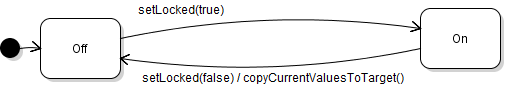
\includegraphics[width=0.75\linewidth]{assets/chpt_impl/sw/AxisManager_onoff}
\end{figure}

\section{Grasp Synergies}
The grasp synergy approach is implemented according to the concepts described in Section \ref{sec:conc:synergy}. The approach are implemented using a gesture page and relative and absolute approach are differentiable by the title of the tabbed page selector, apart from that, the pages look the same.

\subsection{Gesture Parsing}

Gesture parsing is separated into multiple classes. The \textit{GestureParser} class accepts touch events redirected to it by the \textit{GestureView}s on the pages for gesture control. It has a method 
\begin{lstlisting}
public void handleTouchEvent(MotionEvent e);
\end{lstlisting}
which is called from within the \textit{onTouchEvent()} handler of the user interface element. The \textit{GestureParser} is otherwise independent from the user interface element it is invoked by. When a new pointer is encountered, it adds it to a gesture it fits to which is already present on the screen or -- if the pointer is too far away from any existent gesture -- creates a new gesture. If a pointer is removed from the screen, it is also deleted from the gesture it was assigned to. If no pointers are left within the gesture, it is also removed. If an event is received stating a pointer has moved, the pointer location is updated in memory. Upon all of the described actions, the observers of the \textit{GestureParser} are notified. These observers implement the \textit{GestureObserver} interface, which is shown in Listing \ref{lst:impl:gestobs}. It gives the \textit{GestureParser} to notify observers about the addition or removal of a gesture, as well as the case on which a pointer of the gesture has changed its position. 

\begin{lstlisting}[caption={The GestureObserver interface}, label=lst:impl:gestobs]
public interface GestureObserver {
	void onGestureAdd(Gesture g);
	void onGestureRemove(Gesture g);
	void onGestureChanged(Gesture g);
}
\end{lstlisting}

If the pointer count of a gesture changes, the \textit{GestureParser} calls the \textit{onGestureRemove()} method of observers, and then the \textit{onGestureAdd()} method. Both with the same \textit{Gesture} object.

When a gesture is added or its pointer count changes, it is marked as \textit{locked} by the \textit{GestureParser} for the duration of one second. This indicates to dependent classes, that the gesture is new and the data should not yet be used for any control purposes, as the user might still adjust finger positions. This also takes care of the fact that, to add a multi-pointer gesture, the android system calls different events for each pointer subsequently, meaning that to the software it looks as if a one-pointer gesture was added, then a two-pointer gesture and then a three-pointer gesture, if three fingers were laid on the touchscreen. By ignoring gesture input for the first second of a new gesture, the user should have put all fingers onto the screen and can then control the application. Having input by an unwanted gesture may cause unexpected behaviour. In the following the functionality of the three main material classes \textit{Location}, \textit{Pointer} and \textit{Gesture} is explained.

\subsubsection{The Location Class}

The \textit{Location} class represents a two-dimensional vector within the program. It has two coordinates, $x$ and $y$, which can be accessed by \textit{getter methods}. It also offers basic functionality to work with vectors, including addition, subtraction, multiplication with scalars and the scalar-product. All functionality is implemented as expected by common sense. When a mathematical operation is performed using two \textit{Location} objects, the result is returned as a new one, as a \textit{Location} is immutable once it is created.

\begin{lstlisting}[caption={The public interface of the Location class}, label=lst:impl:location]
public class Location {
	public Location(float x, float y);
	
	public float getX();
	public float getY();
	
	public Location add(Location loc);
	public Location substract(Location loc);
	public Location multiply(float c);
	public Location divide(float c);
	
	public double scalarProduct(Location loc);
	
	public double getVectorLength();
	public double distanceTo(Location loc);
	public double getAngleTo(Location loc);
	public Location getTurned(double angleRad);
	public boolean isSame(Location l2);
}
\end{lstlisting}

As visible in Listing \ref{lst:impl:location} multiple advanced operations are also available on \textit{Locations}. \textit{getVectorLength()} returns the length of the vector calculated using the Pythagorean theorem. \textit{getDistanceTo()} is implemented very similar, as it basically calculates the length of the differential vector between the \textit{Location} it is invoked on and the passed second \textit{Location}. Although this could be done by one \textit{substract()} operation and then performing \textit{getVectorLength()} on the result the calculation is directly implemented here for performance reasons.

\begin{lstlisting}[caption={Implementation of getVectorLength() and getDistanceTo()},label=lst:impl:location_length]
public double getVectorLength() {
	return Math.sqrt(Math.pow(x, 2) + Math.pow(y, 2));
}

public double distanceTo(Location loc) {
	return (float)Math.sqrt(Math.pow(loc.x - this.x, 2) + Math.pow(loc.y - this.y, 2));
}
\end{lstlisting}

\textit{getAngleTo()} returns the angle between the \textit{Location} it is invoked on and the one passed as a parameter. Please note that this represents the calculation as defined in Equation \ref{eq:conc:orientation} implemented for arbitrary vectors. This means that the output of this method ranges from $-\pi$ to $\pi$, with positive angles meaning a clockwise rotation from the invoked \textit{Location} to the one passed as a parameter. The reader if referred to Listing \ref{lst:impl:angles} for the implementation of \textit{getAngleTo()}. In Line 4 the determinant of the two combined vectors is calculated and the result is multiplied with $-1$ if the determinant is negative. This could've been written shorter, but for better readability this format was chosen.

\begin{lstlisting}[caption={Implementation of getAngleTo()},label=lst:impl:angles]
public double getAngleTo(Location loc) {
	double val = Math.acos(scalarProduct(loc) / (getVectorLength() * loc.getVectorLength()));
	
	if(x * loc.getY() - y * loc.getX() < 0) {
		val *= -1;
	}

	return val;
}
\end{lstlisting}

Lastly, \textit{getTurned()} returns the current \textit{Location} rotated by an angle of \textit{angleRad}. The angle may range from $-\pi$ to $\pi$, with positive angles meaning a clockwise rotation. \textit{isSame()} is a numerical comparison of the two vectors. Note that floating point numbers are compared here, on which equality comparisons are problematic. This function is used to check for exactly the same values, meaning probably the same location objects.

\subsubsection{The Pointer Class}

Pointers are the contents of \textit{Gestures}. They contain of a \textit{Location}, representing their coordinates on the touch-screen and an id, which is their touch-pointer-id as assigned by the Android operating system. This class was basically introduced to semantically separate the pointer id from the location. The id is needed to identify a pointer within the motion event raised by the operating system. A method is provided to update the location of a pointer, in which a new \textit{Location} object is created.
\begin{lstlisting}[caption={The Pointer class}]
public class Pointer {
	public Pointer(int id, float x, float y);

	public int getId();

	public Location getLocation();
	public void setLocation(float x, float y);
}
\end{lstlisting}

\subsubsection{The Gesture Class}

The \textit{Gesture} class represents a gesture as defined in Section \ref{sec:conc:gestures}. It is basically a set of \textit{Pointer}s with a set of properties. Its public interface is denoted in Listing \ref{lst:impl:gestureclass}.

\begin{lstlisting}[caption={Public interface of the Gesture class},label=lst:impl:gestureclass]
public class Gesture {
	public boolean isLocked();
	public void setLocked(boolean locked);
	
	public void addPointer(Pointer p);
	public void removePointer(Pointer p);
	public int getPointerCount();
	
	public boolean catchesPointer(Pointer p);
	public float getCatchRadius();
	public float getDistanceToCenter(Pointer p);
	
	public Location getCenter();
	public float getSize();
	public double getOrientation();
}
\end{lstlisting}

The first two methods set and query the \textit{locked} state of a gesture, followed by three methods to add and remove pointers, as well as querying the number of currently available pointers in a gesture. Whenever a pointer is added or removed to or from a gesture, the \textit{thumb pointer} is evaluated according to the rules defined in Section \ref{sec:conc:gestures}.
\textit{catchesPointer()} determines whether a new \textit{Pointer} can be added to the gesture. This is done by checking whether the \textit{Pointer}  is within a distance of $2.5$x the size of the gesture around its center. If only one pointer is present in a gesture no size is available. In that case, a size of 1200 is taken as the \textit{catch radius}. \textit{getCenter()}, \textit{getSize()} and \textit{getOrientation()} represent $c(G)$, $s(G)$ and $o(G)$ as defined in section \ref{sec:conc:gestures}.

\subsection{Arm Control}
\label{sec:impl:armcontrol}
\subsubsection{The PointInSpace Class}

The \textit{PointInSpace} class implements functionality as a vector in three dimensions, offering basic operations like adding other \textit{PointInSpace} instances and multiplying with scalars. It is not as elaborated as the \textit{Location} class, but extending the functionality according to \textit{Location} could easily be done if needed.

\begin{lstlisting}[caption={The public interface of PointInSpace}]
public class PointInSpace {
	public PointInSpace(double x, double y, double z);
	
	public double getX();
	public double getY();
	public double getZ();
	
	public PointInSpace add(PointInSpace pw);
	public PointInSpace multiply(double v);
}

\end{lstlisting}

\subsubsection{The CartesianArmManager Class}

The functionality to move the arm (or better: the palm of the robotic hand) in Cartesian space is provided by the \textit{CartesianArmManager}. It accepts positions for the palm and manages the querying of the BioIK service asynchronously in the background. Once it received a result from the IK service it forwards it to the \textit{AxisManager} instance. It holds a list of all joints that shall not be affected by the \textit{CartesianArmManager}, i.e. all joints of the Shadow C5 hand, thus placement of the palm only takes place by moving joints belonging to the Kuka robot arm. It also only updates joints in the \textit{AxisManager} that it shall affect, leaving control to all the other joints to different parts of the software.

\begin{lstlisting}[caption={The public interface of CartesianArmManager}, label=lst:impl:cartarm]
public class CartesianArmManager implements ServiceResponseListener<bio_ik_msgs.GetIKResponse> {
	public static final double Y_MIN = -1.2;
	public static final double Y_MAX = -0.8;
	public static final double X_MIN = -0.2;
	public static final double X_MAX = 0.4;
	public static final double Z_MIN = 1.05;
	public static final double Z_MAX = 1.17;
	
	public static final int MAX_AXIS_CHANGE = 15;
	
	public static CartesianArmManager getInstance();
	
	public void setNode(C5LwrNode node);
	
	
	public boolean goHome();
	public boolean movePalm(PointInSpace offset);
	public boolean movePalmTo(PointInSpace position);
	
	public PointInSpace getPosition();
	
	public void stop();
}
\end{lstlisting}

\begin{wrapfigure}[19]{R}{0.5\linewidth}
	\vspace{-2.2em}
	\caption{\label{fig:impl:cartarmstate}State diagram for the CartesianArmManager update loop}
	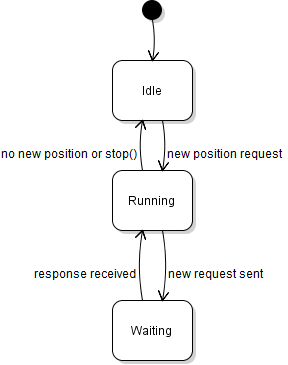
\includegraphics[width=\linewidth]{assets/chpt_impl/sw/CartesianArmManager_loop}
\end{wrapfigure}

Whenever a new target position for the palm is set using \textit{goHome()}, \textit{movePalm()} or \textit{movePalmTo()}, the IK-loop within the \textit{CartesianArmManager} is started. It tries to get solutions from as BioIK service as fast as it can, initiating a new request as soon as one result was received until either no new position was requested or \textit{stop()} was called. Once one of these two cases happen, the loop is stopped and restarted only when a new position is set. Whenever the loop starts a new request, it uses the last set value as target value, values set in between two requests are omitted. Figure \ref{fig:impl:cartarmstate} gives an overview about this process in form of a state diagram.

When a result is returned by the BioIK service it has to go through multiple checks before it is sent to the robot. First, if the \textit{error\_code} field has another value than $0$, the BioIK solver could not find any solution for the queried robot pose, in this case, the \textit{CartesianArmManager} sends the same request to the BioIK service again so it tries to find another solution again. If the \textit{error\_code} field is $0$, the joint angles from the solution are compared to the currently measured state of the robot. When one joint is changed by more than 15 degrees, the solution is rejected as unsafe and a new solution for the same request is queried at the BioIK service. This is done to prevent big movements in joint space, possibly causing unwanted and uncontrollable movements of the robot, potentially causing damage to the robot or its environment. The check for high distances in joint space can be bypassed, which is used when letting the robot go into home position, as this specific position most probably has a bigger distance to the state before than allowed by the check. This means that \textbf{when going to the home position, the user has to watch the robot and has to use caution when using this functionality.} Whenever unwanted movement is observed the user can lift the finger off the safety interlock button to immediately stop any robot movement. As an additional precautionary measure, a hardware emergency switch should be within reach of the operator. When the above checks pass, the joint angled of the arm returned by the BioIK service are written to the \textit{AxisManager} which then sends them to the robot over ROS.

The functionality of the three methods to set new target value is in particular:
\begin{itemize}
	\item \textit{goHome()} sets the target position of the palm to a fixed position which is known to be safely reachable. In this case, it's $p_{home} = \vecthr{0}{y_{min}}{z_{max}}$, which is a position located directly in front of the robot at the border of the table.
	\item \textit{movePalm()} moves the current target position of the palm by \textit{offset} (by adding it to the position returned by \textit{getPosition()}).
	\item \textit{movePalmTo()} overwrites the target position by \textit{position}.
\end{itemize}

\subsection{Grasp Synergies}

An implementation of the grasp synergies is provided by the work of \citeauthor{Bernardino2013} as well as the recorded data matrices representing the matrix of eigenvectors for each of the different grasp synergies. The functionality is bundled within the \textit{GraspSynergy} class. The data files which can be read by the class methods are included into the application as text file resources. A dataset for one grasp consists of two files, which is one file containing the \textit{mean} value or the offset of a grasp ($s_0$ in Section \ref{sec:conc:synergy}) and one file containing the matrix with the matrix data ($S$ in Section \ref{sec:conc:synergy}). Mean files are called \textit{g1mean.txt}, \textit{g2mean.txt} and so on, while the matrix files are called \textit{g1vecs.txt}, \textit{g2vecs.txt} up to \textit{g8vecs.txt}. Originally, these files were named differently when provided by Dr. Norman Hendrich, but due to restrictions of the Android operating system regarding names of resources, they hat to be renamed.
\textit{GraspSynergy} objects are handled and maintained within the \textit{AbsoluteSynergyTouchFragment} and \textit{RelativeSynergyTouchFragment} classes, as they load all grasp synergies, make them selectable within the drop-down list and assign the currently selected synergy object to either the \textit{RelativeSynergyProxy} or the \textit{AbsoluteSynergyProxy}. Thanks to the implementation of \textit{GraspSynergy}, loading synergy data from application resources is done in very few lines as shown in Listing \ref{lst:impl:loadsyn}. The variables \textit{mean\_res} and \textit{vec\_res} are the Android resource IDs for the \textit{mean} and the \textit{vecs} resource file.
\begin{lstlisting}[caption={Loading GraspSynergy data}, label=lst:impl:loadsyn]
GraspSynergy synergy = new GraspSynergy(21);
synergy.parseMatlabSynergyMean(getResources().openRawResource(mean_res));
synergy.parseMatlabSynergyVecs(getResources().openRawResource(vec_res));
\end{lstlisting}

Within the above names fragment classes, loading of synergies is surrounded with error handling for the case loading fails. Additionally, a loaded grasp synergy is added to the drop-down list. All this is encapsulated in a method \textit{loadSynergy()} accepting the synergy name (as displayed) and the corresponding resource IDs. Loading of a synergy is then done in one line as shown in Listing \ref{lst:impl:loadsyncall}.
\begin{lstlisting}[caption={Call to loadSynergy()}, label=lst:impl:loadsyncall]
loadSynergy("Grasp 1", R.raw.g1mean_n, R.raw.g1vecs_n);
\end{lstlisting}

\begin{table}
	\caption{\label{tab:impl:indexjoints}The mapping from array index to joint name}
	\begin{tabular}{|c|c|c|c|c|c|c|c|c|c|c|}
		\hline
		0 & 1 & 2 & 3 & 4 & 5 & 6 & 7 & 8 & 9 & 10 \\
		\hline
		FFJ1 & FFJ2 & FFJ3 & FFJ4 & MFJ1 & MFJ2 & MFJ3 & MFJ4 & RFJ1 & RFJ2 & RFJ3 \\
		\hline
		\hline
		11 & 12 & 13 & 14 & 15 & 16 & 17 & 18 & 19 & 20 & \\
		\hline
		RFJ4 & LFJ1 & LFJ2 & LFJ3 & LFJ4 & THJ1 & THJ2 & THJ3 & THJ4 & THJ5 & \\
		\hline
	\end{tabular}
\end{table}

Once loaded a grasp synergy is used by passing an array of double values to the \textit{toJoints()} method on the \textit{GraspSynergy} object. As described in Section \ref{sec:conc:synergy}, the amplitude values have to be in a range from $-50$ to $50$. The return value of this method is again an array of double values, representing the calculated joint angles in degrees. The mapping of the index within the returned array to the joint name the angle shall be assigned to had to be extracted from code, so it is available in Table \ref{tab:impl:indexjoints} for reasons of completeness. 

The output of \textit{toJoints()} is then passed to \textit{toSafeAbduction()}, which modifies the joint angles in a way that no collisions between fingers are present and returns the modified array of joint angles. These joint angles can then directly be passed to the \textit{AxisManager} which will forward it to the ROS nodes.

\begin{lstlisting}[caption={Example call of toJoints() and toSafeAbduction()}]
double[] jointData =
	_currentSynergy.toSafeAbduction(
		_currentSynergy.toJoints(_amplitudes)
	);
\end{lstlisting}

As this functionality is the same for both the relative and the absolute synergy approach it is bundled within the abstract class \textit{SynergyProxyBase}, which handles the gesture events received by a \textit{GestureParser} and handles the calculation of joint angles using the synergy assigned by the containing fragment class. It analyses the gesture events for changes in size, orientation and position for each gesture and then calls specific calls to abstract methods which shall be implemented by the inheriting classes \textit{AbsoluteSynergyProxy} and \textit{RelativeSynergyProxy} as reactions to changes of a gesture are the only thing unique to the different approaches.
\begin{lstlisting}
protected abstract void handleSizeChange(GestureState oldState, Gesture gesture);
protected abstract void handleLocationChanged(GestureState oldState, Gesture gesture);
protected abstract void handleOrientationChanges(GestureState oldState, Gesture gesture);
\end{lstlisting}
All three methods take the current state of the gesture as well as the state of the gesture from the call before as parameters. The \textit{old state} of active gestures is maintained by the \textit{SynergyProxyBase} implementation. In fact, only \textit{RelativeSynergyProxy} will make use of it, as the absolute synergy control fully relies on the current state of a gesture.

\subsection{Absolute Control}
\label{sec:impl:syn:absc}
The \textit{AbsoluteSynergyProxy} is contained within the \textit{AbsoluteSynergyTouchFragment}, which passes touch events on to the \textit{GestureParser} and registers eht \textit{AbsoluteSynergyProxy} with the \textit{GestureParser} to receive events. It also maintains the list of loaded synergies and assigns the one currently selected to the \textit{AbsoluteSynergyProxy}. Within the three abstract methods of \textit{SynergyProxyBase} that are implemented here current states of gestures are handled. According to their pointer count different actions are made, as two-pointer gestures are used to control the hand synergies, while three-pointer-gestures are used to control the robotic arm. Only the X and Z position of the robot hand palm are used when controlling the arm at the time of writing. The \textit{CartesianArmManager} described in Section \ref{sec:impl:armcontrol} is used to control the position of the palm. 

As values of properties of a gesture shall be mapped linearly to amplitude or position values, a new class is introduced, the \textit{LinearEquation} class. It offers functionality to initialize the parameters of the linear equation by passing it two points between which values shall be mapped as well as the minimum and maximum values that are allowed for the output. Another method available is \textit{calculateClipped()} which calculates the output of the linear equation and clips it to the previously passed minimum and maximum values. The public interface of the \textit{LinearEquation} class can be reviewed in Listing \ref{lst:impl:abs:eq}. Parameters of the linear equation can either be set directly from the constructor or calculated later. This is used when reacting to the screen size, as this value might change at runtime (by changing orientation), so the \textit{calculateParameters()} method is called when the screen size changes and new parameters are calculated.

\begin{lstlisting}[caption={Public interface of the LinearEquation class},label=lst:impl:abs:eq]
public class LinearEquation {
	public LinearEquation(double x1, double y1, double x2, double y2, double min, double max);
	
	public void calculateParameters(double x1, double y1, double x2, double y2);
	public void setLimits(double min, double max);
	
	public double calculateClipped(double x);
}
\end{lstlisting}

To react to screen size changes, \textit{AbsoluteSynergyProxy} implements the method \textit{setCanvasSize()} which is called by the containing fragment class when the screen size changes. Listing \ref{lst:impl:abs:init} shows how the \textit{LinearEquation} objects are initialized first and updated from the \textit{setCanvasSize()} method. The parameters are chosen according to Section \ref{sec:conc:gestures}.

\begin{lstlisting}[caption={Initizlization of LinearEquations for hand and arm}, label=lst:impl:abs:init]
private LinearEquation[] _eqsHand = new LinearEquation[] {
	new LinearEquation(1200, 50, 300, -50, -50, 50),
	new LinearEquation(0, 50, 1000, -50, -50, 50),
	new LinearEquation(-(Math.PI / 2.0), 50, Math.PI / 2.0, -50, -50, 50)
};

private LinearEquation[] _eqsArm = new LinearEquation[] {
	new LinearEquation(300, CartesianArmManager.X_MIN, 1200, CartesianArmManager.X_MAX),
	new LinearEquation(0, CartesianArmManager.Z_MIN, 1000, CartesianArmManager.Z_MAX)
};

public void setCanvasSize(float width, float height) {
	LinearEquation leq = _eqsHand[XPOS_AMPLITUDE];
	leq.calculateParameters(width * 0.25, 50, width * 0.75, -50);
	
	_eqsArm[ARM_X_EQ].calculateParameters(width * 0.25, CartesianArmManager.X_MIN, width * 0.75, CartesianArmManager.X_MAX);
	_eqsArm[ARM_X_EQ].setLimits(CartesianArmManager.X_MIN, CartesianArmManager.X_MAX);
	
	_eqsArm[ARM_Z_EQ].calculateParameters(height * 0.75, CartesianArmManager.Z_MIN, height * 0.25, CartesianArmManager.Z_MAX);
	_eqsArm[ARM_Z_EQ].setLimits(CartesianArmManager.Z_MIN, CartesianArmManager.Z_MAX);
}
\end{lstlisting}

As an example, the usage of the above functionality is shown with the \textit{handleLocationChanged()} event for a gesture. First it is checked whether the pointer count corresponds to that of an arm or a hand control gesture. The coordinates of the gesture are then passed to the corresponding \textit{LinearEquation} objects and the results are written either to an amplitude or the \textit{CartesianArmManager} to update the position of the palm of the hand. The Y coordinate of the hand is maintained the same, as only X and Z coordinates are changed.

\begin{lstlisting}[caption={Example usage of LinearEquation}]
protected void handleLocationChanged(GestureState oldState, Gesture gesture) {
	if(gesture.getPointerCount() == HAND_GEST_POINTER_COUNT) {
		setAmplitude(XPOS_AMPLITUDE, _eqsHand[XPOS_AMPLITUDE].calculateClipped(gesture.getCenter().getX()));
	}
	else if(gesture.getPointerCount() == ARM_GEST_POINTER_COUNT) {
		Location p = gesture.getCenter();
		double x = _eqsArm[ARM_X_EQ].calculateClipped(p.getX());
		double z = _eqsArm[ARM_Z_EQ].calculateClipped(p.getY());
		
		PointInSpace pos = arm.getPosition();
		PointInSpace newPos = new PointInSpace(x, pos.getY(), z);
		arm.movePalmTo(newPos);
	}
}
\end{lstlisting}

\subsection{Relative Control}

The implementation of \textit{RelativeSynergyProxy} is similarly embedded into the environment of \textit{RelativeSynergyTouchFragment}, \textit{GestureParser} and \textit{CartesianArmManager} as the \textit{AbsoluteSynergyProxy}. Within the methods that are called when a gesture changes, the \textit{RelativeChanger} class is used to change amplitudes or the position of the arm relatively to their current position. The parameter \textit{oldState} within all gesture events comes into action here, as only the difference between the old and the current state matters for the calculations. 

The \textit{RelativeChanger} class is initialized with a rate of change and a maximum and minimum value, to which the output shall be clipped. The rate of change is given in two numbers, the one representing the change in the output value corresponding to the change in input value, which is given as a second parameter. This is implemented according to Definition \ref{def:conc:rm} on page \pageref{def:conc:rm}. Additionally it gives the opportunity to invert the changes made by \textit{RelativeChanger} using the \textit{invert} flag during the initialization. Listing \ref{lst:impl:syn:rel} depicts the public interface of the \textit{RelativeChanger} class while Listing \ref{lst:impl:syn:expl} gives an example of its usage according to the one given in Section \ref{sec:impl:syn:absc} to show the main differences between the two approaches. In this approach it's made use of the \textit{movePalm()} method of \textit{CartesianArmManager}, which already changes the position relatively and clips input to the allowed boundaries. Because of this, a \textit{LinearEquation} is used instead of \textit{RelativeChanger} to only get the desired change to the output value, which is then passed to the \textit{CartesianArmManager}.

\begin{lstlisting}[caption={Public interface of the RelativeChanger class},label=lst:impl:syn:rel]
public class RelativeChanger {
	public RelativeChanger(double valueChange, double inputChange, boolean invert, double min, double max);
	public void setRateBySpan(double valueChange, double inputChange, boolean invert, double min, double max);
	public double getChangedClipped(double oldValue, double inputChange);
}
\end{lstlisting}

\begin{lstlisting}[caption={Example usage of RelativeChanger in RelativeSynergyProxy},label=lst:impl:syn:expl]
RelativeChanger[] _changers = new RelativeChanger[] {
	new RelativeChanger(50, 1200, false, -50, 50),
	new RelativeChanger(50, 1200, false, -50, 50),
	new RelativeChanger(40, Math.PI, false, -50, 50)
};

LinearEquation armXEq = new LinearEquation(0, 0, 2200, CartesianArmManager.X_MAX - CartesianArmManager.X_MIN);
LinearEquation armZEq = new LinearEquation(0, 0, -1000, CartesianArmManager.Z_MAX - CartesianArmManager.Z_MIN);

protected void handleLocationChanged(GestureState oldState, Gesture gesture) {
	if(gesture.getPointerCount() == HAND_GEST_POINTER_COUNT) {
		double xChange = gesture.getCenter().getX() - oldState.getCenter().getX();
		
		setAmplitude(XPOS_AMPLITUDE, _changers[XPOS_AMPLITUDE].getChangedClipped(getAmplitude(XPOS_AMPLITUDE), xChange));
	}
	else if(gesture.getPointerCount() == ARM_GEST_POINTER_COUNT) {
		Location old = oldState.getCenter();
		Location newLoc = gesture.getCenter();
		Location offset = newLoc.substract(old);
		
		PointInSpace armoffset = new PointInSpace(
			armXEq.calculate(offset.getX()),
			0,
			armZEq.calculate(offset.getY())
		);
		
		CartesianArmManager.getInstance().movePalm(armoffset);
	}
}
\end{lstlisting}


\section{Direct Fingertip Mapping (DFTM)}
\label{sec:impl:dfmt}

The \textit{direct fingertip mapping} (DFTM) is mainly implemented using the \textit{DfmtProxy} and \textit{FingertipPointer} classes, in which most of the functionality is contained. The \textit{DftmProxy} class implements the \textit{Singleton} pattern. Its instance is used from the \textit{FingertipFragment} class which offers the user interface for this approach and forwards all touch events of the user interface to the \textit{DftmProxy}. For BioIK service interactions, the \textit{DftmProxy} class directly depends on the \textit{C5LwrNode} which offers the functionality needed to request joint angle solutions for a set of given fingertip positions.

The \textit{FingertipPointer} class stores information about one fingertip that is laid onto the touch screen, which is it's position in screen coordinates, the name of the effector (also called \textit{link}) which is controlled by this fingertip and the coordinates of the pointer in meters. The latter is stored within this class for convenience reasons and is calculated whenever the screen coordinates of the pointer change. Having the world coordinates available reduces the computational load when writing the information to the screen on the \textit{FingertipFragment}. Both coordinates originate in the top-left corner of the screen. In addition to the position of the pointer a flag is stored whether the pointer is currently available on the screen, i.e.~a finger is currently positioned on the screen controlling this pointer.

For the calculation of the world coordinates in centimeters to be correct, the screen metrics, namely the width, height and number of dots per inch (DPI) have to be set once they are known to the user interface (\textit{FingertipFragment}). The coordinates are calculated using Equation \ref{eq:conc:dftm:world} from page \pageref{eq:conc:dftm:world} with $r$ being the dots per inch as set by the user interface class.

The effector controlled by a \textit{FingertipPointer} is determined by the order in which the fingertips are laid down onto the screen. At the moment, at most three fingertips may be controlled using this approach. The first finger put down onto the screen controls the thumb (\textit{thtip}), the second controls the first finger (\textit{fftip}) and the third the second or middle finger \textit{mftip}. This should usually map the finger controlled to the actual finger of the controller's hand. Fingers can be lifted during operation. If the lifted finger was the last finger laid down onto the screen, the pointer is removed from the list of pointers sent to the BioIK service. If the finger was not the last one laid down onto the screen, the corresponding \textit{FingertipPointer} is markes as \textit{not present}, which means that no finger is currently controlling its position but it is still included in BioIK service calls. Once a finger is put onto the approximate position where it was lifted, the pointer is again marked as \textit{present} and its position is updated periodically. The public interface of the \textit{FingertipPointer} class is shown in Listing \ref{lst:impl:dftm:fingertip}.

\begin{lstlisting}[caption={Public interface of the FingertipPointer class},label=lst:impl:dftm:fingertip]
public class FingertipPointer {
	public FingertipPointer(String effectorName, Location screenLoc, int id);
	
	public String getEffectorName():
	
	public int getPointerId();
	public void setPointerId(int pointerId);
	
	
	public Location getScreenLocation();
	public void setScreenLocation(Location screenLocation);
	
	public Location getWorldLocation();
	public void setWorldLocation(Location worldLocation);
	
	public boolean isPresent();
	public void setPresent(boolean present);
}
\end{lstlisting}

Once a new position for a fingertip is found, the \textit{update loop} is started. The update loop for this approach is very similar to the one of the \textit{CartesianArmManager} depicted in Figure \ref{fig:impl:cartarmstate} on page \pageref{fig:impl:cartarmstate}. The \textit{DftmProxy} requests new solutions for the current pointers' locations until either no pointers are registered anymore or the \textit{DftmProxy} is disabled using the \textit{setEnabled()} method. Once a new solution is returned to \textit{DftmProxy}, it is also checked against a maximum movement of 15 degrees on a per-joint basis, solutions with a too big displacement are discarded and a new solution is requested.

To request a solution the desired locations of the fingertips in three-dimensional space have to be calculated first. As the position of the fingertips is known in meters from the top-left corner of the screen, the simple calculations described in Section \ref{sec:conc:dftm} can be done using no more conversions. The \textit{PointInSpace} class offers all functionality needed for these calculations. The base vector and the two spanning vectors are currently defined as fixed values and shown in Listing \ref{lst:impl:dftm:vect}. Listing \ref{lst:impl:dftm:mapping} shows how the mapping from two-dimensional screen coordinates into three-dimensional coordinates is performed.

\begin{lstlisting}[caption={Vectors used for planar mapping},label=lst:impl:dftm:vect]
PointInSpace surfaceBase = new PointInSpace(0.0, -1.25, 1.2);
PointInSpace surfaceYBaseVect = new PointInSpace(0, 1, 0);
PointInSpace surfaceXBaseVect = new PointInSpace(-1, 0, 0);
\end{lstlisting}

\begin{lstlisting}[caption={Mapping of points from two into three dimensions},label=lst:impl:dftm:mapping]
FingertipPointer p = _pointers[i];

PointInSpace wloc = surfaceBase
	.add(surfaceXBaseVect.multiply(p.getWorldLocation().getX()))
	.add(surfaceYBaseVect.multiply(p.getWorldLocation().getY()));
\end{lstlisting}

Once this calculation has been done for all pointers current present, the request at the BioIK service is made. In addition to the fingertip locations, the \textit{C5LwrNode} class adds a \textit{MinimalDisplacementGoal} to the request to indicate to the service that a solution with minimal displacement of all joints is desirable. Additionally, a \textit{OrientationGoal} is added, forcing the palm of the robotic hand into a top-down orientation. Otherwise, the IK solver could find solutions where the fingertips are at the correct positions but were placed there from the bottom, which is correct in principle, but neither a expected nor a desired solution.

The safety interlock button on the screen sets the enabled flag of the \textit{DftmProxy} which is redirected to the \textit{AxisManager}. This means that once the safety interlock button is released, no movement is done by the robot. If an IK request is still pending and the result is returned after the button has been released, the solution is discarded since the \textit{AxisManager} does not accept new joint angles. At the time of writing it is not possible to move the base vector of the plane fingertips are mapped to. Thus actions are limited to a very small workspace. Functionality to \textit{scroll} the workspace can be implemented by changing the base vector, but it has to made sure that the movement is safe and no unexpected joint angle changes occur.